\chapter{随机过程与样本路径}
\label{chap:stochastic-processes-and-sample-paths}

设想一台温度传感器每分钟读一次数，连续记录一整天；把这件事重复许多天，桌上就摊开了一摞曲线。对这摞曲线可以提出性质很不相同的问题。早上八点的读数超过$20$度的概率是多少？八点与八点零五分的读数同时偏高的概率是多少？某一天的曲线是否曾经越过$30$度，若越过，是哪一分钟第一次越过？到中午为止已经看到的读数，对下午的走势能说明什么？第一个问题只涉及一个时刻，第二个问题涉及几个时刻的共同变化，第三个问题涉及整条曲线，第四个问题则涉及随时间增长的信息。

本章把这四类问题放进同一个数学对象：定义在同一概率空间上的一族随机变量。第~\ref{sec:spp-families-paths}节先说明固定时刻与固定一次实现分别得到什么，并用相同边缘、不同相关的几个序列说明为什么必须记录多时刻的联合规律；同时指出，即使联合规律完全确定，“曲线是否连续”这类整条路径的问题也未必能在乘积结构中提出。第~\ref{sec:spp-information}节给时间索引加上信息结构，规定在每个时刻哪些事件已经可以判定，由此定义适应过程和停时。第~\ref{sec:spp-construction}节回答怎样从可以写下的规则得到过程：有时间先后时逐步使用条件规律，没有先后时指定一组相容的有限维分布；随后区分“构造出了坐标族”与“得到了想要的路径性质”，引入版本、不可区分和Kolmogorov连续性准则。

后三节把索引从时间推广到一般位置和集合，作为上述构造思路的实例。高斯过程用均值函数与协方差函数规定任意位置组上的联合高斯读数；交换序列的依赖来自共享的随机背景而不是时间转移；随机概率测度的每次实现本身就是一个概率分布，Dirichlet过程是其中最重要的例子。这三节可以独立阅读，第~\ref{chap:discrete-time-stochastic-processes}章与第~\ref{chap:continuous-time-stochastic-processes}章只依赖前三节建立的共同语言。

本章使用的条件期望、塔式性质、概率核及其复合、条件分布的存在条件，都取自概率空间部分；需要时我们在当地重述所用的结论与条件，完整的定义与证明可参考\BookChapterRef{chap:conditional-expectation}{卷二“条件期望与条件分布”章}。

% 第4章第1节：随机变量族与样本路径（共同概率空间、两种读法、有限维分布、路径规律）。

\section{随机变量族与样本路径}
\label{sec:spp-families-paths}

本节确定研究对象。我们从几种重复读数出发，说明为什么一族随机变量必须定义在同一个概率空间上；再分别固定索引和固定一次实现，得到随机变量与样本路径这两种读法。随后用相同边缘、不同相关的序列说明单时刻分布为何不够，引入有限维分布，并把整条路径看成函数空间中的随机元素，检查哪些关于路径的问题可以在这个框架中提出。

\subsection{索引、状态与共同概率空间}
\label{sec:spp-index-state-space}

\paragraph{三种重复读数}
设一台传感器反复测量同一个量，第$n$次读数记为$X_n$，测量噪声$\varepsilon_1,\varepsilon_2,\ldots$相互独立，都服从$\mathcal N(0,\sigma^2)$。下面三种模型都产生一列读数。
\begin{enumerate}
  \item 独立读数：被测量是固定常数$\theta$，$X_n=\theta+\varepsilon_n$。
  \item 共享背景：被测量$\Theta\sim\mathcal N(0,\tau^2)$本身随机（例如当天的环境条件），与全部噪声独立，$X_n=\Theta+\varepsilon_n$。
  \item 误差累计：仪器每次把新误差叠加到上一次读数上，$S_0=0$，$S_n=\varepsilon_1+\cdots+\varepsilon_n$。
\end{enumerate}
第二种模型中每个$X_n$都服从$\mathcal N(0,\tau^2+\sigma^2)$；若在第一种模型中取$\theta=0$，再把噪声方差换成$\tau^2+\sigma^2$，单次读数的分布就与第二种完全相同。只看一次读数，无法区分这两种情形。

区别出现在涉及多次读数的问题上。在共享背景模型中，$\operatorname{Cov}(X_m,X_n)=\tau^2$对$m\ne n$成立，前$n$次读数的平均满足
\[
  \operatorname{Var}\Bigl(\frac1n\sum_{i=1}^nX_i\Bigr)=\tau^2+\frac{\sigma^2}{n},
\]
无论读多少次，平均值的方差都不低于$\tau^2$；而独立读数的平均方差$(\tau^2+\sigma^2)/n$随$n$趋于零。累计模型中$\operatorname{Cov}(S_m,S_n)=\sigma^2\min(m,n)$，相邻读数共享此前的全部误差。这些量都同时涉及第$m$次与第$n$次读数，所以“第$m$次读数”和“第$n$次读数”必须是同一次实验结果$\omega$的两个函数：只有这样，$\{X_1>0,\ X_2>0\}$才是一个有意义的事件。若只给出每次读数各自的分布，就无法回答两次读数是否共享$\Theta$。

\paragraph{随机过程的定义}
因此，研究一族读数时，先固定一个概率空间，再把每个读数写成它上面的随机变量。索引不必是测量轮次，也可以是连续时间、平面上的位置，甚至是可测集合；取值也不必是实数。下面的定义只要求每个坐标可测。

\begin{definition}[随机过程]
\label{def:spp-process}
设$(\Omega,\mathcal F,\mathbb P)$是概率空间，$T$是非空集合，$(E,\mathcal E)$是可测空间。若对每个$t\in T$，映射$X_t:\Omega\to E$都是$\mathcal F/\mathcal E$可测的，就称映射族$X=(X_t)_{t\in T}$为定义在$(\Omega,\mathcal F,\mathbb P)$上、以$T$为\term{索引集}、以$E$为\term{状态空间}的\term{随机过程}（stochastic process）。$T\subseteq\mathbb Z$时也称$X$为\term{随机序列}（random sequence）。
\end{definition}

每个坐标的可测性保证单个读数有分布：$\mathbb P(X_t\in B)$对每个$B\in\mathcal E$有定义，$\mathbb P\circ X_t^{-1}$是$E$上的概率测度。随机对象、推前测度与联合分布的一般讨论可参考\BookChapterRef{chap:probability-models}{卷二“一般概率模型与随机对象”章}；本章需要的只是：同一概率空间上的有限个可测映射$(X_{t_1},\ldots,X_{t_m})$合起来仍是取值于乘积空间$(E^m,\mathcal E^{\otimes m})$的可测映射，因而有联合分布。

几个常见索引可以帮助辨认这个定义的范围。$T=\mathbb N_0$时，$X$是按整数时刻记录的序列；$T=[0,\infty)$时，$X$在每个实数时刻都有值；$T$为平面区域$D$时，$(X_x)_{x\in D}$是一个随机场，例如一片区域上同一时刻的气温；$T$为可测集合族$\mathcal E$时，$(G(A))_{A\in\mathcal E}$可以是一族随机质量，第~\ref{sec:spp-random-measures}节研究的随机概率测度就属于这一类。

\paragraph{固定索引与固定结果}
随机过程是两个变量的函数$(t,\omega)\mapsto X_t(\omega)$，固定其中任何一个都得到有用的对象。固定$t$，得到随机变量$\omega\mapsto X_t(\omega)$，它描述时刻$t$的读数在各次实验之间怎样变化；固定$\omega$，得到一个从$T$到$E$的普通函数。

\begin{definition}[样本路径]
\label{def:spp-sample-path}
对随机过程$X=(X_t)_{t\in T}$和固定的$\omega\in\Omega$，函数$t\mapsto X_t(\omega)$称为$X$的一条\term{样本路径}（sample path），记作$X_\cdot(\omega)$。它是函数集合$E^T=\{x:T\to E\}$中的一个元素。
\end{definition}

图~\ref{fig:spp-two-views}把这两种读法画在一起。左图中每条灰线是一次实验的完整记录，蓝线是其中一条；沿横轴看一条线，读到的是一次实现随时间怎样变化。竖虚线固定一个时刻，它与各条路径的交点是该时刻在不同实验中的读数；把$2000$条路径在两个时刻的交点做成直方图，就得到右图中$S_{10}$与$S_{30}$的分布。竖切片越往后越宽，这是方差$\operatorname{Var}(S_n)=n$的直观形态；但右图的两个直方图没有记录同一条路径在两个时刻的值怎样配对，这部分信息只能沿横向读出。

\begin{figure}[htbp]
  \centering
  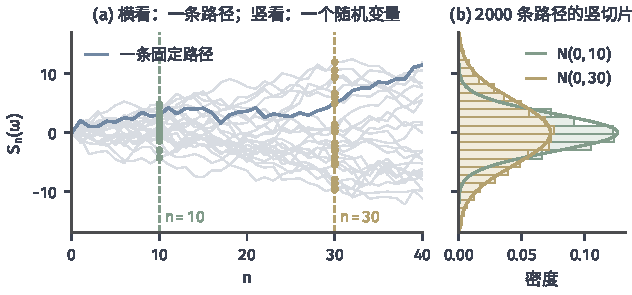
\includegraphics[width=107mm]{figures/03-optimization-evolution-and-signals/02-processes-and-trajectory-evolution/matplotlib/spp-two-views/figure.pdf}
  \caption{随机过程的两种读法。模型为高斯随机游走$S_0=0$，$S_n=\xi_1+\cdots+\xi_n$，$\xi_i$独立服从$\mathcal N(0,1)$，共模拟$2000$条路径（固定随机种子）。(a)灰线为其中$24$条路径，蓝线为一条固定路径；竖虚线固定时刻$n=10$与$n=30$，圆点为前$25$条路径在这两个时刻的值。(b)全部$2000$条路径在这两个时刻的直方图，曲线为精确分布$\mathcal N(0,10)$与$\mathcal N(0,30)$。}
  \label{fig:spp-two-views}
\end{figure}

\begin{example}[三次抛硬币的两种读法]
\label{ex:spp-three-coins}
抛一枚均匀硬币三次，$\Omega=\{\mathrm H,\mathrm T\}^3$，八个结果等可能。令正面记$+1$、反面记$-1$，$\xi_k(\omega)$为第$k$次的记号，$S_0=0$，$S_n=\xi_1+\cdots+\xi_n$，$n=1,2,3$。固定$\omega=\mathrm{HTH}$，样本路径是$(S_0,S_1,S_2,S_3)=(0,1,0,1)$，这是一个确定的四元数组。固定$n=2$，$S_2$在$\mathrm{HH}*$上取$2$，在$\mathrm{HT}*$与$\mathrm{TH}*$上取$0$，在$\mathrm{TT}*$上取$-2$，其中$*$表示第三次任意；因而$\mathbb P(S_2=2)=\mathbb P(S_2=-2)=1/4$，$\mathbb P(S_2=0)=1/2$。前者回答“这一次发生了什么”，后者回答“在时刻$2$可能发生什么、各有多大概率”。
\end{example}

\paragraph{时间、状态与路径的三个判断}
描述一个过程时，有三个彼此独立的判断。第一，索引是离散还是连续：$T=\mathbb N_0$称为离散时间，$T$为实数区间称为连续时间。第二，状态是离散还是连续：$E$可以是有限集、整数集，也可以是$\mathbb R^d$。第三，在连续时间且状态空间带有拓扑时，样本路径是连续的还是带有跳跃。“连续时间”只说明每个实数时刻都有值，并不说明取值连续，更不说明路径连续。

图~\ref{fig:spp-taxonomy}给出四个代表。(a)的简单随机游走在整数时刻取整数值；(b)的自回归序列$Y_{n+1}=0.8Y_n+0.6\eta_{n+1}$在整数时刻取实数值；(c)的计数路径在每个实数时刻都有值，却只取整数，并在随机时刻跳升$1$；(d)的Brownian路径在连续时间中连续变化，但放大后仍然粗糙。连续时间、实数取值的过程也可以有跳跃，例如在计数过程的每次跳跃处加上一个随机实数幅度；在$\mathbb R^d$上运行的Markov链Monte Carlo算法则是离散时间、连续状态的过程。后两章按时间索引组织，正是因为离散时间与连续时间提出的技术问题不同：前者只涉及可数个时刻，后者要处理不可数个时刻，路径性质和可测性需要额外条件。

\begin{figure}[htbp]
  \centering
  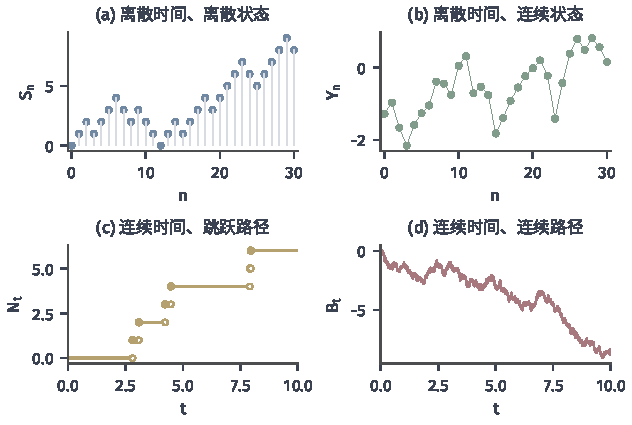
\includegraphics[width=107mm]{figures/03-optimization-evolution-and-signals/02-processes-and-trajectory-evolution/matplotlib/spp-taxonomy/figure.pdf}
  \caption{按索引与路径类型区分的四类过程，均为固定随机种子下的单条模拟路径。(a)简单对称随机游走，每步$\pm1$；(b)平稳自回归序列$Y_{n+1}=0.8Y_n+0.6\eta_{n+1}$，$\eta_n$独立服从$\mathcal N(0,1)$；(c)速率为$1$的计数过程，实心点为跳跃时刻的取值，空心点为跳跃前的左极限；(d)用$4000$个等距小步近似的Brownian路径。时间是离散还是连续，与状态、路径是否连续是分开的判断。}
  \label{fig:spp-taxonomy}
\end{figure}

\subsection{有限维分布与路径规律}
\label{sec:spp-fdd-path-law}

\paragraph{相同边缘、不同依赖}
上一小节的共享背景例子已经说明，单次读数的分布不能决定平均值的行为。下面把这个现象做成一个干净的对照：三个序列的每个坐标都服从$\mathcal N(0,1)$，只有依赖结构不同。取$\rho=0.8$，令$\varepsilon_n,\eta_n,\Theta$均为相互独立的标准高斯变量。
\begin{enumerate}
  \item 独立序列：$X_n=\varepsilon_n$，$\operatorname{Cov}(X_m,X_n)=0$，$m\ne n$。
  \item 自回归序列：$Y_0=\varepsilon_0$，$Y_{n+1}=\rho Y_n+\sqrt{1-\rho^2}\,\eta_{n+1}$。由归纳，$\operatorname{Var}(Y_{n+1})=\rho^2+(1-\rho^2)=1$，且$\operatorname{Cov}(Y_n,Y_{n+k})=\rho^k$。
  \item 共享背景序列：$Z_n=\sqrt\rho\,\Theta+\sqrt{1-\rho}\,\varepsilon_n$，$\operatorname{Var}(Z_n)=\rho+(1-\rho)=1$，$\operatorname{Cov}(Z_m,Z_n)=\rho$，$m\ne n$。
\end{enumerate}
三个序列在任何单个时刻都无法区分。前$100$项平均的方差却分别为
\begin{align*}
  \text{独立序列：}\quad&\frac1{100}=0.01,\\
  \text{自回归序列：}\quad&\frac1{100^2}\Bigl(100+2\sum_{k=1}^{99}(100-k)\rho^k\Bigr)\approx0.086,\\
  \text{共享背景序列：}\quad&\rho+\frac{1-\rho}{100}=0.802 .
\end{align*}
第二个数来自把$\operatorname{Var}(\sum_iY_i)=\sum_{i,j}\rho^{|i-j|}$按间隔$k=|i-j|$分组。图~\ref{fig:spp-same-marginals}显示了差别的来源：独立序列在灰带内来回跳动；自回归序列有记忆，相关随间隔几何衰减；共享背景序列整条路径围绕一个随机水平波动，任意两项的相关都是$0.8$，这个水平不会因为多读几次而被平均掉。

\begin{figure*}[htbp]
  \centering
  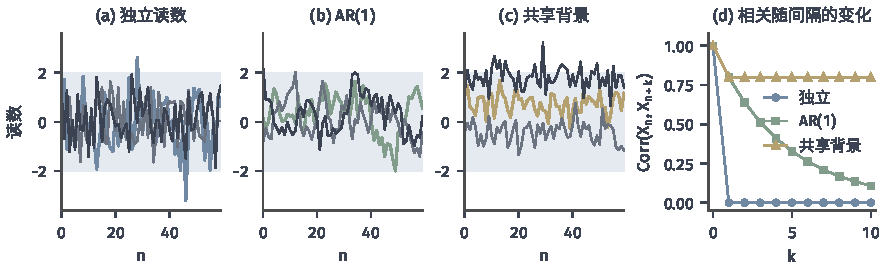
\includegraphics[width=150mm]{figures/03-optimization-evolution-and-signals/02-processes-and-trajectory-evolution/matplotlib/spp-same-marginals/figure.pdf}
  \caption{三个单时刻边缘都为$\mathcal N(0,1)$的序列。(a)--(c)各画三条长$60$的模拟路径（固定随机种子），浅蓝带为$\pm2$，即单个$\mathcal N(0,1)$读数约$95\%$的范围：(a)独立序列；(b)自回归序列，$\rho=0.8$；(c)共享背景序列，$Z_n=\sqrt{0.8}\,\Theta+\sqrt{0.2}\,\varepsilon_n$。(d)理论相关系数随间隔$k$的变化：独立序列在$k\ge1$时为$0$，自回归序列为$0.8^k$，共享背景序列恒为$0.8$。三者前$100$项平均的方差依次为$0.01$、约$0.086$与$0.802$。}
  \label{fig:spp-same-marginals}
\end{figure*}

\paragraph{有限维分布}
要区分这三个序列，至少需要记录任意几个时刻的联合分布。对一般过程，这就是下面的定义。

\begin{definition}[有限维分布]
\label{def:spp-fdd}
设$X=(X_t)_{t\in T}$是取值于$(E,\mathcal E)$的随机过程。对每个正整数$m$和互不相同的$t_1,\ldots,t_m\in T$，令
\[
  \mu_{t_1,\ldots,t_m}(B)=\mathbb P\bigl((X_{t_1},\ldots,X_{t_m})\in B\bigr),\qquad B\in\mathcal E^{\otimes m}.
\]
全体这样的概率测度称为$X$的\term{有限维分布}（finite-dimensional distributions）。
\end{definition}

上面三个序列的有限维分布都是均值为零的高斯分布，区别只在协方差矩阵：独立序列为单位矩阵，自回归序列的$(i,j)$元为$\rho^{|t_i-t_j|}$，共享背景序列的非对角元全为$\rho$。

同一过程的有限维分布不能随意指定，它们之间有两条必然的关系。设$\pi$是$\{1,\ldots,m\}$的一个排列，记$\sigma_\pi(x_1,\ldots,x_m)=(x_{\pi(1)},\ldots,x_{\pi(m)})$。

\begin{theorem}[有限维分布的相容关系]
\label{thm:spp-fdd-consistency}
任意随机过程的有限维分布满足：
\begin{enumerate}
  \item 重排相容：$\mu_{t_{\pi(1)},\ldots,t_{\pi(m)}}=\mu_{t_1,\ldots,t_m}\circ\sigma_\pi^{-1}$；
  \item 边缘相容：对$m\ge2$与$B\in\mathcal E^{\otimes(m-1)}$，$\mu_{t_1,\ldots,t_m}(B\times E)=\mu_{t_1,\ldots,t_{m-1}}(B)$。
\end{enumerate}
\end{theorem}

\begin{proof}
两条都是同一个事件的两种写法。对$B\in\mathcal E^{\otimes m}$，$(X_{t_{\pi(1)}},\allowbreak\ldots,\allowbreak X_{t_{\pi(m)}})\in B$当且仅当$(X_{t_1},\allowbreak\ldots,\allowbreak X_{t_m})\in\sigma_\pi^{-1}(B)$，两边取概率即得第一条。$(X_{t_1},\allowbreak\ldots,\allowbreak X_{t_m})\in B\times E$当且仅当$(X_{t_1},\allowbreak\ldots,\allowbreak X_{t_{m-1}})\in B$，因为最后一个坐标总在$E$中，取概率即得第二条。
\end{proof}

相容关系说的是：同一个“两时刻问题”，不论直接用两时刻分布回答，还是从三时刻分布中积掉第三个坐标再回答，答案必须一样。第~\ref{sec:spp-kolmogorov-extension}小节讨论反方向的问题：给定一族满足这两条的分布，是否一定存在过程以它们为有限维分布。

\paragraph{路径作为随机元素}
有限维分布一次只看有限个时刻。“路径是否曾越过某个水平”这类问题涉及整条路径，需要把路径本身当作一个随机对象。把每个$\omega$映到它的样本路径，得到映射
\[
  X:\Omega\to E^T,\qquad \omega\mapsto X_\cdot(\omega).
\]
要谈论$X$的分布，先要在$E^T$上选定$\sigma$代数。最自然的选择是让每个坐标读取$\pi_t:x\mapsto x(t)$都可测的最小$\sigma$代数，即\term{乘积$\sigma$代数}（product sigma-algebra）$\mathcal E^{\otimes T}$。它也由形如
\begin{equation}
  C=\bigl\{x\in E^T:\ (x(t_1),\ldots,x(t_m))\in B\bigr\},\qquad t_1,\ldots,t_m\in T,\ B\in\mathcal E^{\otimes m}
  \label{eq:spp-cylinder}
\end{equation}
的集合生成，这类集合称为\term{柱集}（cylinder set）：它只在有限个时刻检查路径是否满足某项条件，其余时刻不加限制。图~\ref{fig:spp-cylinder}中三个时刻各设一道“闸门”，柱集就是同时穿过三道闸门的全部路径；闸门之间路径怎样走，柱集不管。

\begin{figure}[htbp]
  \centering
  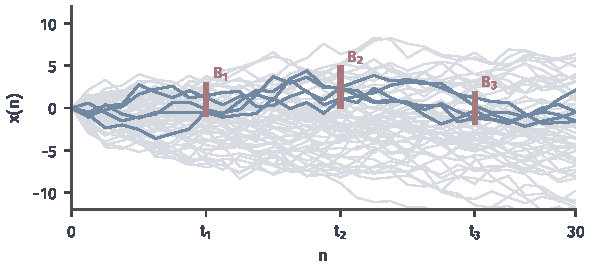
\includegraphics[width=100mm]{figures/03-optimization-evolution-and-signals/02-processes-and-trajectory-evolution/matplotlib/spp-cylinder/figure.pdf}
  \caption{柱集$\{x:\ x(t_1)\in B_1,\ x(t_2)\in B_2,\ x(t_3)\in B_3\}$。红色竖条为三个时刻上的区间$B_1=[-1,3]$、$B_2=[0,5]$、$B_3=[-2,2]$；$60$条高斯随机游走路径（固定随机种子）中，同时穿过三个区间的画成蓝色，其余为灰色。柱集只约束这三个时刻的取值。}
  \label{fig:spp-cylinder}
\end{figure}

\begin{theorem}[路径映射的可测性与路径规律]
\label{thm:spp-path-law}
设$X=(X_t)_{t\in T}$是取值于$(E,\mathcal E)$的一族映射。
\begin{enumerate}
  \item 路径映射$X:(\Omega,\mathcal F)\to(E^T,\mathcal E^{\otimes T})$可测，当且仅当每个$X_t$可测，即$X$是随机过程。
  \item 若$X$是随机过程，则推前测度$P_X=\mathbb P\circ X^{-1}$是$(E^T,\mathcal E^{\otimes T})$上的概率测度，称为$X$的\term{路径规律}（law of the process）。两个随机过程（可以定义在不同的概率空间上）具有相同的有限维分布，当且仅当它们的路径规律相同。
\end{enumerate}
\end{theorem}

\begin{proof}
(1) 由于$\pi_t\circ X=X_t$，若$X$可测，则每个$X_t$作为可测映射的复合可测。反之，若每个$X_t$可测，则$\{B\subseteq E^T:\ X^{-1}(B)\in\mathcal F\}$是$\sigma$代数，并包含每个$\pi_t^{-1}(A)$，因为$X^{-1}(\pi_t^{-1}(A))=X_t^{-1}(A)\in\mathcal F$；它因而包含这些集合生成的$\mathcal E^{\otimes T}$。

(2) 柱集\eqref{eq:spp-cylinder}的概率是$P_X(C)=\mu_{t_1,\ldots,t_m}(B)$，所以路径规律相同蕴含有限维分布相同。反过来，两个柱集的交仍是柱集：把两组时刻合并，各自的条件改写到合并后的坐标上即可。于是柱集族是对有限交封闭、生成$\mathcal E^{\otimes T}$的集合族。两个概率测度若在这样的集合族上相等，就在它生成的$\sigma$代数上相等（这是$\pi$--$\lambda$定理的推论，可参考\BookChapterRef{chap:measures}{卷二“测度”章}）。有限维分布相同意味着两个路径规律在全部柱集上相等，因而处处相等。
\end{proof}

这一定理说明，在乘积$\sigma$代数的层面上，“过程的规律”与“全部有限维分布”是同一份信息。它也划定了这份信息的边界：只有属于$\mathcal E^{\otimes T}$的路径事件，其概率才由有限维分布决定。

\paragraph{可数个坐标决定的事件}
索引可数时，乘积$\sigma$代数已经包含许多关于整条路径的事件。设$T=\mathbb N_0$，$E=\mathbb R$。“路径曾超过$c$”是可数并$\bigcup_n\{x:\ x(n)>c\}$；“路径收敛”可以写成$\{\limsup_nx(n)=\liminf_nx(n)\in\mathbb R\}$，而$\limsup_nx(n)=\inf_m\sup_{n\ge m}x(n)$是可测函数的可数次上下确界。这些事件的概率都由有限维分布决定，第~\ref{chap:discrete-time-stochastic-processes}章研究的回返、命中和极限问题都在这个框架内。

索引不可数时情况不同。关键在于下面的观察：乘积$\sigma$代数中的每个事件只依赖可数个坐标。

\begin{theorem}[乘积$\sigma$代数中的事件由可数个坐标决定]
\label{thm:spp-countable-coordinates}
设$A\in\mathcal E^{\otimes T}$。则存在可数集合$S\subseteq T$，使得对任意$x,y\in E^T$，只要$x$与$y$在$S$上相等，就有$x\in A\Leftrightarrow y\in A$。
\end{theorem}

\begin{proof}
记$\mathcal D$为具有上述性质的集合$A\subseteq E^T$组成的族。柱集\eqref{eq:spp-cylinder}属于$\mathcal D$，取$S=\{t_1,\ldots,t_m\}$即可。若$A\in\mathcal D$，对应可数集$S$，则$A^c$用同一个$S$也满足要求。若$A_k\in\mathcal D$对应$S_k$，令$S=\bigcup_kS_k$，它仍可数；当$x,y$在$S$上相等时，它们在每个$S_k$上相等，于是对每个$k$有$x\in A_k\Leftrightarrow y\in A_k$，从而$x\in\bigcup_kA_k\Leftrightarrow y\in\bigcup_kA_k$。所以$\mathcal D$是包含柱集的$\sigma$代数，含有$\mathcal E^{\otimes T}$。
\end{proof}

取$T=[0,1]$，$E=\mathbb R$。连续函数全体$C[0,1]$不属于$\mathbb R^{\otimes[0,1]}$：若它属于，设对应的可数集为$S$，取$t^\ast\in[0,1]\setminus S$；零函数连续，而函数$\mathbb I_{\{t=t^\ast\}}$与零函数在$S$上相等，却在$t^\ast$处不连续，与定理矛盾。同样的论证表明$\{x:\ \sup_{t\in[0,1]}x(t)>0\}$也不在乘积$\sigma$代数中。因此，对连续时间过程，单凭有限维分布甚至不能提出“路径连续的概率是多少”这个问题。第~\ref{sec:spp-versions}小节将说明怎样通过选取合适的过程版本绕过这一障碍。

% 第4章第2节：历史信息与适应过程（滤过、自然滤过、适应性、停时）。

\section{历史信息与适应过程}
\label{sec:spp-information}

上一节的有限维分布与路径规律是“事后”的描述：它们把整段记录当作一次给定的结果来看。可是许多问题要求站在某个时刻，只用已经发生的记录作判断：预测下一步时能用哪些读数，什么时候停止监测，下一步的投入能否依赖尚未揭晓的噪声。本节给时间索引加上信息结构。滤过规定每个时刻已经可以判定的事件，适应性检查过程的当前值是否已知，停时则把“何时停下”也纳入同样的要求。第~\ref{chap:discrete-time-stochastic-processes}章与第~\ref{chap:continuous-time-stochastic-processes}章中的Markov性质、鞅性质和随机累计，都相对于这里指定的信息来陈述。

本节的索引集$T$是$\mathbb R$的子集并沿用实数的顺序，典型情形是$T=\mathbb N_0$或$T=[0,\infty)$。

\subsection{滤过与适应性}
\label{sec:spp-filtration-adapted}

\paragraph{信息随时间增长}
回到示例~\ref{ex:spp-three-coins}的三次抛硬币。在时刻$1$，我们只知道第一次的结果；能够判定是否发生的事件，恰好是那些由第一次结果决定的事件，例如“第一次是正面”。在样本空间上看，这相当于把八个结果按第一次的结果分成两块：我们知道$\omega$落在哪一块，却不知道它在块内的位置。到时刻$2$，分块细化为按前两次结果划分的四块；到时刻$3$，每块只剩一个结果。

图~\ref{fig:spp-filtration-layers}把这四层分块从上到下排开，块内数字是随机游走$S_n$在该块上的取值。每一层的块都是上一层某一块的再分割，因为新的记录只会增加、不会抹去已知的结果。另一个值得注意的事实是：$S_n$在第$n$层的每一块内取常数，所以到时刻$n$为止的记录足以确定$S_n$；而$S_3$在第$2$层的块内并不是常数，例如$\mathrm{HH}*$块中$S_3$可能是$3$也可能是$1$，在时刻$2$还不能确定。

\begin{figure}[htbp]
  \centering
  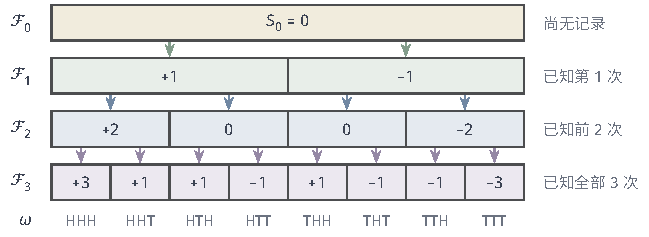
\includegraphics[width=110mm]{figures/03-optimization-evolution-and-signals/02-processes-and-trajectory-evolution/tikz/spp-filtration-layers/figure.pdf}
  \caption{三次抛硬币的自然滤过。最下一行是八个等可能的结果$\omega$；第$n$行把它们按前$n$次结果分块，每一块是$\mathcal F_n$中不可再分的事件，$\mathcal F_n$由这些块的全部并组成。块内数字是随机游走$S_n$（正面$+1$、反面$-1$）在该块上的取值；箭头表示每一层都是上一层的细分。}
  \label{fig:spp-filtration-layers}
\end{figure}

\paragraph{滤过与自然滤过}
在一般概率空间上，“时刻$t$能够判定的事件”组成一个子$\sigma$代数，记作$\mathcal F_t$。信息只增不减，于是得到一列递增的子$\sigma$代数。

\begin{definition}[滤过与自然滤过]
\label{def:spp-filtration}
设$(\Omega,\mathcal F,\mathbb P)$是概率空间，$T\subseteq\mathbb R$。一族子$\sigma$代数$(\mathcal F_t)_{t\in T}$若满足
\[
  \mathcal F_s\subseteq\mathcal F_t\subseteq\mathcal F,\qquad s,t\in T,\ s\le t,
\]
就称为\term{滤过}（filtration），$(\Omega,\mathcal F,(\mathcal F_t)_{t\in T},\mathbb P)$称为带滤过的概率空间。对随机过程$X=(X_t)_{t\in T}$，
\[
  \mathcal F^X_t=\sigma(X_s:\ s\in T,\ s\le t)
\]
是由截至时刻$t$的记录生成的$\sigma$代数，$(\mathcal F^X_t)_{t\in T}$称为$X$的\term{自然滤过}（natural filtration）。
\end{definition}

滤过描述的是“谁知道什么”，不一定由所研究的过程本身生成。一个观测者可能从一开始就掌握某个初始信息，也可能同时看到另一路信号；这时他的信息族比$X$的自然滤过更大。同一个过程可以相对于不同的滤过研究，后面会看到，结论可能因此改变。

\paragraph{适应过程}
有了滤过，就可以说一个随机量“在时刻$t$已经可知”：它关于$\mathcal F_t$可测，意味着对每个可测集$B$，事件“它落在$B$中”在时刻$t$已经可以判定。

\begin{definition}[适应过程]
\label{def:spp-adapted}
若对每个$t\in T$，$X_t$关于$\mathcal F_t$可测，就称过程$X=(X_t)_{t\in T}$适应于滤过$(\mathcal F_t)_{t\in T}$，也称$X$是\term{适应过程}（adapted process）。
\end{definition}

每个过程都适应于自己的自然滤过，而且自然滤过是使它适应的最小滤过：若$X$适应于$(\mathcal G_t)$，则对$s\le t$有$X_s$关于$\mathcal G_s\subseteq\mathcal G_t$可测，所以生成的$\sigma$代数$\mathcal F^X_t\subseteq\mathcal G_t$。在有限样本空间上，若$\mathcal F_n$由一个有限分块生成，那么$X_n$关于$\mathcal F_n$可测，当且仅当$X_n$在每一块上取常数：每个事件$\{X_n=x\}$都必须是若干整块的并。图~\ref{fig:spp-filtration-layers}中$S_n$在第$n$层每块上为常数，正是适应性的直观形态；而$S_{n+1}$通常不在第$n$层的块上取常数，所以“下一时刻的位置”这个过程$(S_{n+1})_n$不适应于自然滤过。

\begin{example}[按块平均的预测]
\label{ex:spp-block-average}
在图~\ref{fig:spp-filtration-layers}的有限样本空间上，给定$\mathcal F_n$的条件期望就是在第$n$层的每一块内对等可能结果取平均。例如在时刻$1$预测$S_3$：$\mathrm H**$块中$S_3$的四个值为$3,1,1,-1$，平均为$1$；$\mathrm T**$块中为$1,-1,-1,-3$，平均为$-1$。所以$\mathbb E[S_3\mid\mathcal F_1]=S_1$。同样地，在第$2$层的$\mathrm{HH}*$块中$S_3$取$3$或$1$，平均为$2=S_2$。在这个模型中，用截至当前的记录预测未来位置，最好的均方预测就是当前位置；把第$1$层的块平均再在第$0$层平均，得到$\mathbb ES_3=0$，这正是塔式性质在分块上的样子：先在细块内平均，再在粗块内平均，等于直接在粗块内平均。
\end{example}

\paragraph{同一过程，不同信息}
下面的例子说明，同一个过程在两种滤过下给出不同的预测，二者之间的关系由条件期望的塔式性质刻画。

\begin{example}[共享背景下的两个观测者]
\label{ex:spp-two-observers}
沿用第~\ref{sec:spp-index-state-space}小节的共享背景读数$X_n=\Theta+\varepsilon_n$，$\Theta\sim\mathcal N(0,\tau^2)$，噪声$\varepsilon_n$独立服从$\mathcal N(0,\sigma^2)$且与$\Theta$独立。观测者甲只看到读数，信息为自然滤过$\mathcal F_n=\sigma(X_1,\ldots,X_n)$；观测者乙事先知道$\Theta$，信息为$\mathcal G_n=\sigma(\Theta,X_1,\ldots,X_n)$。读数过程同时适应于这两个滤过，并且$\mathcal F_n\subseteq\mathcal G_n$。

对乙而言，$\varepsilon_{n+1}$与$\mathcal G_n$独立且均值为零，所以
\[
  \mathbb E[X_{n+1}\mid\mathcal G_n]=\Theta+\mathbb E[\varepsilon_{n+1}\mid\mathcal G_n]=\Theta .
\]
对甲而言，$\varepsilon_{n+1}$同样与$\mathcal F_n$独立，于是$\mathbb E[X_{n+1}\mid\mathcal F_n]=\mathbb E[\Theta\mid\mathcal F_n]$。为了算出它，令$\bar X_n=\frac1n\sum_{i=1}^nX_i$，$c=n\tau^2/(n\tau^2+\sigma^2)$，并考虑残差$R=\Theta-c\bar X_n$。直接计算
\[
  \operatorname{Cov}(R,X_i)=\tau^2-c\Bigl(\tau^2+\frac{\sigma^2}{n}\Bigr)=0,\qquad i=1,\ldots,n .
\]
$(R,X_1,\ldots,X_n)$是独立高斯变量的线性组合，因而联合高斯；联合高斯向量中不相关的分量相互独立，所以$R$与$\mathcal F_n$独立，$\mathbb E[R\mid\mathcal F_n]=\mathbb ER=0$。于是
\[
  \mathbb E[X_{n+1}\mid\mathcal F_n]=c\,\bar X_n=\frac{n\tau^2}{n\tau^2+\sigma^2}\,\bar X_n .
\]
甲把读数平均值向零收缩，因为他不知道这个平均值中有多少来自$\Theta$、多少来自噪声；读数越多，收缩系数越接近$1$。

两个预测满足塔式性质$\mathbb E\bigl[\mathbb E[X_{n+1}\mid\mathcal G_n]\bigm|\mathcal F_n\bigr]=\mathbb E[X_{n+1}\mid\mathcal F_n]$：把乙的预测$\Theta$按甲的信息再平均一次，正好得到甲的预测。预测误差也可以直接比较。乙的均方误差是$\mathbb E\varepsilon_{n+1}^2=\sigma^2$；甲的误差$X_{n+1}-c\bar X_n=R+\varepsilon_{n+1}$，均方误差为
\[
  \sigma^2+\operatorname{Var}(R)=\sigma^2+\frac{\tau^2\sigma^2}{n\tau^2+\sigma^2},
\]
其中$\operatorname{Var}(R)=\tau^2-c^2(\tau^2+\sigma^2/n)=\tau^2(1-c)$。取$\tau=\sigma=1$、$n=4$，甲的预测为$0.8\bar X_4$，均方误差$1.2$；乙的预测为$\Theta$，均方误差$1$。信息越多，最优均方预测的误差越小，这是塔式性质下条件方差分解的一个具体实例。
\end{example}

\paragraph{性质要相对于滤过说明}
滤过的选择不仅影响预测的数值，也影响过程是否具有某种性质。第~\ref{chap:discrete-time-stochastic-processes}章将正式定义鞅与Markov性质；这里只用它们的直观含义看一个对照。设$\xi_1,\xi_2,\ldots$独立，等概率取$\pm1$，$S_0=0$，$S_n=\xi_1+\cdots+\xi_n$。相对于自然滤过$\mathcal F_n=\sigma(\xi_1,\ldots,\xi_n)$，下一步的条件平均不变：
\[
  \mathbb E[S_{n+1}\mid\mathcal F_n]=S_n+\mathbb E\xi_{n+1}=S_n ,
\]
这正是“公平博弈”的性质。现在设想一个提前一步知道结果的观测者，他的信息为$\mathcal H_n=\sigma(\xi_1,\ldots,\xi_{n+1})$。$S$仍然适应于$(\mathcal H_n)$，但
\[
  \mathbb E[S_{n+1}\mid\mathcal H_n]=S_{n+1}\ne S_n ,
\]
对这个观测者而言，博弈不再公平。因此，“$S$是鞅”这句话必须带上滤过才有意义。

Markov性质也一样。在示例~\ref{ex:spp-two-observers}中，乙给定$\mathcal G_n$时下一读数的条件分布是$\mathcal N(\Theta,\sigma^2)$，只通过$\Theta$依赖已有信息；甲给定$\mathcal F_n$时，下一读数的条件分布依赖全部读数的平均值$\bar X_n$，单凭当前读数$X_n$并不足够。若把$(n,\bar X_n)$一并放进状态，甲面对的就是一个只依赖当前状态的递推。状态是否“足够”同样是相对于信息结构而言的，第~\ref{chap:discrete-time-stochastic-processes}章将在一般条件下讨论这一点。

\subsection{随机时刻与停止时刻}
\label{sec:spp-stopping-times}

\paragraph{何时停下由记录决定}
监测常常在读数第一次越过阈值时结束，赌徒可能在赢够一定数额时离场，迭代算法在误差指标首次低于容差时终止。这些停止时刻都是随机的：不同的实验结果在不同的时刻停下。随机时刻是取值于$T\cup\{\infty\}$的映射$\tau:\Omega\to T\cup\{\infty\}$，$\tau(\omega)=\infty$表示永不停止。一条停止规则能够实际执行，必须满足一个要求：在每个时刻$t$，只凭截至$t$的记录就能判断是否已经停下。

\paragraph{停时的定义}
把这个要求写成可测性条件，就得到下面的定义。

\begin{definition}[停时]
\label{def:spp-stopping-time}
设$(\mathcal F_t)_{t\in T}$是滤过。随机时刻$\tau:\Omega\to T\cup\{\infty\}$若对每个$t\in T$满足
\[
  \{\tau\le t\}\in\mathcal F_t ,
\]
就称为相对于该滤过的\term{停时}（stopping time），也称停止时刻。
\end{definition}

离散时间$T=\mathbb N_0$时，这个条件等价于对每个$n$有$\{\tau=n\}\in\mathcal F_n$。若$\{\tau\le n\}\in\mathcal F_n$对每个$n$成立，则$\{\tau=n\}=\{\tau\le n\}\setminus\{\tau\le n-1\}$，后一个集合属于$\mathcal F_{n-1}\subseteq\mathcal F_n$；反之，$\{\tau\le n\}=\bigcup_{k=0}^n\{\tau=k\}$，每一项属于$\mathcal F_k\subseteq\mathcal F_n$。离散情形下“现在是否恰好停下”与“现在是否已经停下”可以互相判定；连续时间中单点时刻的事件往往概率为零，定义因此采用$\{\tau\le t\}$。

常数时刻$\tau\equiv t_0$是停时，因为$\{\tau\le t\}$是$\varnothing$或$\Omega$。若$\tau,\sigma$都是停时，则$\tau\wedge\sigma=\min(\tau,\sigma)$与$\tau\vee\sigma=\max(\tau,\sigma)$也是停时：
\begin{gather*}
  \{\tau\wedge\sigma\le t\}=\{\tau\le t\}\cup\{\sigma\le t\},\\
  \{\tau\vee\sigma\le t\}=\{\tau\le t\}\cap\{\sigma\le t\},
\end{gather*}
右边都属于$\mathcal F_t$。特别地，$\tau\wedge n$是一个不超过$n$的停时，第~\ref{chap:discrete-time-stochastic-processes}章常用它把可能无界的停时截断。

\paragraph{首次命中与全程最高点}
最常见的停时是首次命中时刻。设$S$是随机游走，取整数阈值$a>0$，令
\[
  \tau_a=\inf\{n\ge0:\ S_n\ge a\},\qquad \inf\varnothing=\infty .
\]
对每个$n$，
\[
  \{\tau_a\le n\}=\bigcup_{k=0}^n\{S_k\ge a\}\in\mathcal F_n ,
\]
因为每个$S_k$（$k\le n$）关于$\mathcal F_k\subseteq\mathcal F_n$可测。同样的论证表明：若$X$适应于$(\mathcal F_n)$，$B$是可测集，则首次进入时刻$\inf\{n:\ X_n\in B\}$是停时。图~\ref{fig:spp-stopping-vs-peak}(a)中，路径在$n=7$第一次达到阈值$3$，停止的决定当场就能做出，之后的灰色部分与判断无关。

与之对照，考虑在$\{0,1,\ldots,N\}$上首次达到全程最大值的时刻$\sigma=\min\{n\le N:\ S_n=\max_{k\le N}S_k\}$。取$N=2$并逐一列出四种结果：$\mathrm{HH}$时路径为$0,1,2$，$\sigma=2$；$\mathrm{HT}$时为$0,1,0$，$\sigma=1$；$\mathrm{TH}$时为$0,-1,0$，最大值$0$首次出现在$n=0$，$\sigma=0$；$\mathrm{TT}$时$\sigma=0$。于是$\{\sigma=1\}=\{\xi_1=+1,\ \xi_2=-1\}$，它依赖第二次的结果，不属于只含$\varnothing$、$\{\xi_1=+1\}$、$\{\xi_1=-1\}$与$\Omega$的$\mathcal F_1$。所以$\sigma$不是停时。图~\ref{fig:spp-stopping-vs-peak}(b)显示了一般原因：到$n=6$为止，两条路径的历史完全相同，$n=5$是迄今的最高点；它是否是全程最高点，取决于之后走低还是走高。

\begin{figure}[htbp]
  \centering
  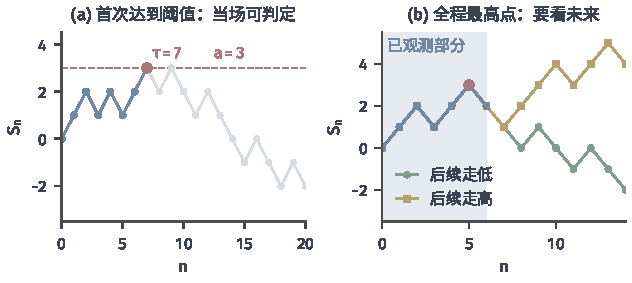
\includegraphics[width=107mm]{figures/03-optimization-evolution-and-signals/02-processes-and-trajectory-evolution/matplotlib/spp-stopping-vs-peak/figure.pdf}
  \caption{停时与非停时。两图均为步长$\pm1$的教学路径。(a)首次达到阈值$a=3$的时刻$\tau=7$（红点）：是否停止只需看到当前为止的蓝色部分。(b)两条路径在浅蓝区域（$n\le6$）内完全相同，$n=5$（红点）是迄今最高点；绿色延续中它仍是全程最高点，黄色延续中则不是。“全程最高点的时刻”要看未来才能判定。}
  \label{fig:spp-stopping-vs-peak}
\end{figure}

\paragraph{定义不提供期望等式}
停时的定义只保证停止规则不偷看未来，并不保证停止后各种平均关系依然成立。下面的倍投策略是标准的警示。

\begin{example}[倍投策略]
\label{ex:spp-doubling}
设$\xi_1,\xi_2,\ldots$独立，等概率取$\pm1$，代表一枚公平硬币。赌徒第$k$轮押注$2^{k-1}$，累计盈亏为$M_0=0$，$M_n=\sum_{k=1}^n2^{k-1}\xi_k$。每轮押注在开局前已经确定，硬币公平，所以$\mathbb E[M_{n+1}\mid\mathcal F_n]=M_n+2^n\mathbb E\xi_{n+1}=M_n$，对每个固定的$n$都有$\mathbb EM_n=0$。赌徒在第一次赢时离场：$\tau=\min\{k:\ \xi_k=+1\}$。它是首次命中时刻，因而是停时；又$\mathbb P(\tau>n)=2^{-n}$，所以$\tau<\infty$几乎必然成立。

在离场时刻，前$\tau-1$轮共输$1+2+\cdots+2^{\tau-2}=2^{\tau-1}-1$，第$\tau$轮赢$2^{\tau-1}$，故$M_\tau=1$恒成立，$\mathbb EM_\tau=1\ne0=\mathbb EM_0$。截断后的情形则不同：若$\tau\le n$，则$M_{\tau\wedge n}=1$；若$\tau>n$，则前$n$轮全输，$M_{\tau\wedge n}=-(2^n-1)$。于是
\[
  \mathbb EM_{\tau\wedge n}=(1-2^{-n})\cdot1+2^{-n}\cdot\bigl(-(2^n-1)\bigr)=0 .
\]
$M_{\tau\wedge n}$几乎必然收敛到$M_\tau=1$，期望却一直是$0$：概率$2^{-n}$的巨额亏损恰好抵消了其余情形的收益，在极限中消失。
\end{example}

这个例子说明，停时之后的期望等式需要额外条件来排除“小概率、大损失”的情形。第~\ref{chap:discrete-time-stochastic-processes}章在离散时间中建立可选停止定理及其条件，并用停时陈述强Markov性质。连续时间中，即使是首次命中时刻也需要额外的路径与滤过条件才能保证是停时，例如路径右连续、滤过满足适当的右连续性；这些条件及相应的可积性要求由第~\ref{chap:continuous-time-stochastic-processes}章补充。

% 第4章第3节：过程的构造与路径版本（逐步核构造、Kolmogorov扩张、版本与连续版本）。

\section{过程的构造与路径版本}
\label{sec:spp-construction}

前两节都假定过程已经给定。实际建模时，手中往往只有一些可以写下的规则：“从当前历史出发，下一步按某个条件分布抽取”，或者“任意有限个位置上的读数服从某个联合分布”。本节回答两个问题。第一，这些有限的规则能否拼成同一个概率空间上的一整族随机变量？有时间先后的情形用条件规律逐步构造，没有先后的情形用相容的有限维分布构造。第二，构造出来的坐标族是否具有我们想要的路径性质？上一节已经看到，连续时间下有限维分布不足以回答路径问题；我们将引入版本与不可区分这两种“相等”，并用Kolmogorov连续性准则得到连续版本。

\subsection{由条件规律逐步构造}
\label{sec:spp-kernel-construction}

\paragraph{逐步抽样的规则}
先看一个依赖整段历史的例子。罐中起初有一个标$1$的球和一个标$0$的球。每次随机摸出一个球，记下标号，把它放回，再放入一个同标号的新球。这个过程称为\term{Pólya罐}（Pólya urn）。记第$n$次的标号为$X_n$，前$n-1$次中摸到$1$的次数为$k$，此时罐中有$k+1$个$1$球、$n-k$个$0$球，于是
\[
  \mathbb P(X_n=1\mid X_1=x_1,\ldots,X_{n-1}=x_{n-1})=\frac{1+k}{n+1}.
\]
下一步的条件分布依赖全部历史中$1$的个数，而不只依赖上一步的结果。图~\ref{fig:spp-polya-tree}把前三步画成一棵树：每条边上是给定此前历史的条件概率，一条从根到叶的路径的概率是沿途条件概率的乘积。

\begin{figure}[htbp]
  \centering
  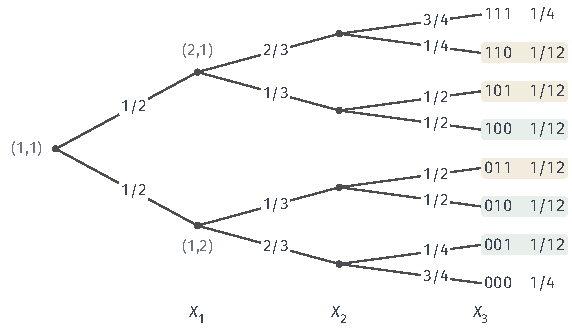
\includegraphics[width=97mm]{figures/03-optimization-evolution-and-signals/02-processes-and-trajectory-evolution/tikz/spp-polya-tree/figure.pdf}
  \caption{Pólya罐前三步的逐步构造。灰色数对是罐中$1$球与$0$球的个数，边上数字是给定此前历史时下一步标号的条件概率，右侧为三步路径及其概率（沿途条件概率之积）。含两个$1$的三条路径（黄底）概率都是$1/12$，含一个$1$的三条路径（绿底）也都是$1/12$：路径概率只依赖$1$的个数，不依赖出现的先后。}
  \label{fig:spp-polya-tree}
\end{figure}

一般地，设状态空间为可测空间$(E,\mathcal E)$，给定初始分布$\mu$和一列概率核$K_n$，$n\ge1$，其中$K_n$从历史空间$E^n$到$E$：输入历史$(x_0,\ldots,x_{n-1})$，输出下一状态的分布$K_n(x_0,\ldots,x_{n-1};\cdot)$。概率核要求对每个历史输出一个概率测度，并且对每个可测集$C$，$K_n(\cdot\,;C)$是历史的可测函数。前$n$步的联合分布由逐层“先抽历史、再按核抽下一步”给出：
\begin{equation}
  \begin{aligned}
  P_n(\mathrm dx_0,\ldots,\mathrm dx_n)
  &=\mu(\mathrm dx_0)\,K_1(x_0;\mathrm dx_1)\,K_2(x_0,x_1;\mathrm dx_2)\\
  &\qquad\cdots K_n(x_0,\ldots,x_{n-1};\mathrm dx_n).
  \end{aligned}
  \label{eq:spp-kernel-chain}
\end{equation}
这个记号的严格含义来自概率空间部分的核积分定理：给定空间$S$上的概率测度$\nu$与从$S$到$E$的概率核$K$，存在唯一的概率测度$\nu\otimes K$定义在$S\times E$上，使$(\nu\otimes K)(B\times C)=\int_BK(s;C)\,\nu(\mathrm ds)$。取$S=E^n$、$\nu=P_{n-1}$、$K=K_n$，就由$P_{n-1}$得到$P_n=P_{n-1}\otimes K_n$；从$P_0=\mu$出发归纳，即得式~\eqref{eq:spp-kernel-chain}。

\paragraph{相容性来自归一化}
逐步构造的有限维分布自动相容。对$B\in\mathcal E^{\otimes n}$，
\[
  P_n(B\times E)=\int_BK_n(x_0,\ldots,x_{n-1};E)\,P_{n-1}(\mathrm dx)=P_{n-1}(B),
\]
所以积掉最后一步就回到前一步的分布；这里用到的只是每个核的总质量为$1$。在任何以$P_n$为前$n+1$个坐标联合分布的过程中，$K_n(X_0,\ldots,X_{n-1};\cdot)$都是$X_n$给定历史的一个条件分布。

逐步构造覆盖了大多数离散时间模型。若$K_n(x_0,\ldots,x_{n-1};\cdot)=P(x_{n-1},\cdot)$只依赖最后一个状态，且核$P$不随$n$变化，就得到时间齐次的\term{Markov链}（Markov chain），第~\ref{chap:discrete-time-stochastic-processes}章研究它的回返与长期性质。例如两状态链从$X_0=0$出发，转移概率$P(0,\{0\})=0.9$、$P(0,\{1\})=0.1$，则$\mathbb P(X_1=0,X_2=1)=0.9\times0.1=0.09$。第~\ref{sec:spp-fdd-path-law}小节的自回归序列也是这样构造的，它的核是$K(y;\cdot)=\mathcal N(\rho y,1-\rho^2)$。Pólya罐则是核依赖整段历史的例子。

\begin{example}[Pólya罐的路径概率]
\label{ex:spp-polya-path}
推广到罐中起初有$a>0$个$1$球、$b>0$个$0$球（允许非整数，此时把个数理解为权重）。对任一长为$n$、含$k$个$1$的序列$(x_1,\ldots,x_n)$，按式~\eqref{eq:spp-kernel-chain}把沿途条件概率相乘。分母依次是$a+b,a+b+1,\ldots,a+b+n-1$，与序列无关；在摸到$1$的那些步上，分子依次是$a,a+1,\ldots,a+k-1$，在摸到$0$的那些步上依次是$b,b+1,\ldots,b+n-k-1$，次序只影响这些因子出现在哪一步，不影响乘积。记上升阶乘$c^{(j)}=c(c+1)\cdots(c+j-1)$，$c^{(0)}=1$，得到
\begin{equation}
  \mathbb P(X_1=x_1,\ldots,X_n=x_n)=\frac{a^{(k)}\,b^{(n-k)}}{(a+b)^{(n)}} .
  \label{eq:spp-polya-path}
\end{equation}
取$a=b=1$、$n=3$：$k=2$时为$1\cdot2\cdot1/(2\cdot3\cdot4)=1/12$，$k=3$时为$1\cdot2\cdot3/24=1/4$，与图~\ref{fig:spp-polya-tree}一致。路径概率只依赖$1$的个数，这一对称性将在第~\ref{sec:spp-exchangeable}节成为交换性的出发点。
\end{example}

\paragraph{可数步的过程}
式~\eqref{eq:spp-kernel-chain}给出了任意有限步的分布。但“最终被吸收”“频率收敛”这些问题涉及无穷多步，需要整条无穷序列上的一个概率测度。下面的定理保证这样的测度存在且唯一，而且不需要状态空间具有任何拓扑结构。

\begin{theorem}[Ionescu-Tulcea定理]
\label{thm:spp-ionescu-tulcea}
设$(E_n,\mathcal E_n)$，$n\ge0$，是任意可测空间，$\mu$是$E_0$上的概率测度，$K_n$是从$E_0\times\cdots\times E_{n-1}$到$E_n$的概率核，$n\ge1$。则在$\Omega=\prod_{n\ge0}E_n$及其乘积$\sigma$代数上存在唯一的概率测度$P$，使对每个$n$，前$n+1$个坐标的联合分布等于式~\eqref{eq:spp-kernel-chain}中的$P_n$。坐标过程$X_n(x)=x_n$在$P$下以$\mu$为初始分布，以$K_n$为各步的条件分布。
\end{theorem}

上述构造结论可参考文献\scite{math-kallenberg2021probability}。

唯一性已由定理~\ref{thm:spp-path-law}给出：两个这样的测度有相同的有限维分布。存在性的思路如下，可作为补充阅读。

\begin{proof}[存在性的证明思路]
对只依赖前$m+1$个坐标的柱集$A=B\times\prod_{n>m}E_n$，令$P(A)=P_m(B)$。由上面的相容性，同一个柱集换用更多坐标表示时值不变，所以$P$在柱集代数上有定义且有限可加。按Carathéodory延拓定理，只需验证：若柱集$A_1\supseteq A_2\supseteq\cdots$满足$P(A_k)\ge\varepsilon>0$，则$\bigcap_kA_k\ne\varnothing$。

设$A_k$依赖前$m_k+1$个坐标。对$n\ge0$，令$h_k^{(n)}(x_0,\ldots,x_n)$为“已知前$n+1$个坐标后$A_k$发生的条件概率”：$n\ge m_k$时它就是$A_k$的示性函数，$n<m_k$时用核$K_{n+1},\ldots,K_{m_k}$把后续坐标逐层积掉。于是
\begin{gather*}
  h_k^{(n)}(x_0,\ldots,x_n)=\int h_k^{(n+1)}(x_0,\ldots,x_n,y)\,K_{n+1}(x_0,\ldots,x_n;\mathrm dy),\\
  \int h_k^{(0)}\,\mathrm d\mu=P(A_k)\ge\varepsilon .
\end{gather*}
由$A_k$递减，$h_k^{(n)}$关于$k$递减，记极限为$g^{(n)}$。对上面两式令$k\to\infty$，被积函数取值于$[0,1]$，由控制收敛定理，$g^{(n)}$满足同样的递推，且$\int g^{(0)}\,\mathrm d\mu\ge\varepsilon$。于是存在$x_0$使$g^{(0)}(x_0)\ge\varepsilon$；而若$g^{(n)}(x_0,\ldots,x_n)\ge\varepsilon$，递推式说明存在$x_{n+1}$使$g^{(n+1)}(x_0,\ldots,x_{n+1})\ge\varepsilon$。归纳得到序列$x=(x_0,x_1,\ldots)$。对每个$k$取$n\ge m_k$，有$\mathbb I_{A_k}(x)=h_k^{(n)}(x_0,\ldots,x_n)\ge g^{(n)}(x_0,\ldots,x_n)\ge\varepsilon>0$，所以$x\in A_k$。
\end{proof}

证明中每一步只用到核的积分和总质量为$1$，从未用到$E_n$的拓扑。这与下一小节的Kolmogorov扩张定理形成对照：那里没有核可用，紧性代替了核的作用。

\paragraph{标准Borel空间上的两种描述}
反方向的问题是：给定一个序列的规律，能否把它写成“初始分布加历史条件核”？这需要每一步的条件分布能拼成概率核，即正则条件分布存在。在\term{标准Borel空间}（standard Borel space）上这总是可以做到的；标准Borel空间是指其可测结构同构于某个完备可分度量空间的Borel子集，$\mathbb R^d$、有限集和可数集都属于此类。于是在标准Borel状态空间上，“序列在$E^{\mathbb N_0}$上的规律”与“初始分布加历史条件核”是同一模型的两种等价描述，后者中的核在几乎处处意义下唯一。第~\ref{chap:discrete-time-stochastic-processes}章正是在这个意义下用转移核刻画离散时间过程。

\subsection{由相容有限维分布构造}
\label{sec:spp-kolmogorov-extension}

\paragraph{没有先后的索引}
逐步构造依赖时间顺序：先有过去，才谈得上给定过去的下一步。可是平面上的温度场、以输入位置为索引的随机函数都没有自然的先后。这时能够直接写下的是：任意有限个位置上的读数服从什么联合分布。于是问题变成第~\ref{sec:spp-fdd-path-law}小节问题的逆向版本：给定一族有限维分布，是否存在一个过程以它们为有限维分布？

为了把重排相容性吸收进记号，用索引的有限子集代替有序元组。对有限集$J\subseteq T$，记$E^J$为从$J$到$E$的函数全体，配乘积$\sigma$代数；对有限集$J\subseteq K$，记$\pi_{K,J}:E^K\to E^J$为限制映射$x\mapsto x|_J$，记$\pi_J:E^T\to E^J$为从整条路径到$J$上坐标的限制。

\begin{definition}[相容的有限维分布族]
\label{def:spp-consistent-family}
设对$T$的每个非空有限子集$J$给定$(E^J,\mathcal E^{\otimes J})$上的概率测度$\mu_J$。若对任意有限集$J\subseteq K\subseteq T$都有
\[
  \mu_K\circ\pi_{K,J}^{-1}=\mu_J ,
\]
就称$\{\mu_J\}$是相容的。
\end{definition}

用函数$x:J\to E$而不是有序元组表示坐标后，排列坐标只是换一种列举方式，不会产生新的测度，第~\ref{sec:spp-fdd-path-law}小节的两条相容关系合并为这一条。若过程$X$存在，令$\mu_J$为$(X_t)_{t\in J}$的分布，由定理~\ref{thm:spp-fdd-consistency}，这族分布必然相容。

\paragraph{相容性保证柱集概率有定义}
有了相容族，可以尝试在柱集上定义$P(\pi_J^{-1}(B))=\mu_J(B)$。困难在于同一个柱集可以用不同的坐标集表示：若$\pi_J^{-1}(B)=\pi_{J'}^{-1}(B')$，两种表示给出的值必须一样。相容性恰好保证这一点。令$K=J\cup J'$，则$\pi_{K,J}^{-1}(B)$与$\pi_{K,J'}^{-1}(B')$是同一个柱集在$K$上的底，二者相等，于是
\[
  \mu_J(B)=\mu_K\bigl(\pi_{K,J}^{-1}(B)\bigr)=\mu_K\bigl(\pi_{K,J'}^{-1}(B')\bigr)=\mu_{J'}(B').
\]
用同样的办法把有限个不相交的柱集放到共同的坐标集上，可知$P$在柱集代数上有限可加。剩下的是可数可加性，这一步需要状态空间的正则性。

\begin{theorem}[Kolmogorov扩张定理]
\label{thm:spp-kolmogorov-extension}
设$(E,\mathcal E)$是标准Borel空间，$T$是任意非空集合，$\{\mu_J\}$是相容的有限维分布族。则在$(E^T,\mathcal E^{\otimes T})$上存在唯一的概率测度$P$，使对每个有限集$J\subseteq T$都有$P\circ\pi_J^{-1}=\mu_J$。坐标过程$X_t(x)=x(t)$在$(E^T,\mathcal E^{\otimes T},P)$上以$\{\mu_J\}$为有限维分布。
\end{theorem}

上述构造结论可参考文献\scite{math-kallenberg2021probability}。

这个结论称为\term{Kolmogorov扩张定理}（Kolmogorov extension theorem）。唯一性仍由定理~\ref{thm:spp-path-law}给出。存在性的证明较长，下面只记录它的结构，作为补充阅读。

\begin{proof}[存在性的证明思路]
可以把$E$看成某个完备可分度量空间$\bar E$中的Borel子集。完备可分度量空间上的概率测度在Borel集上可以用紧子集从内部逼近，所以对每个$\mu_J$和$B\in\mathcal E^{\otimes J}$，存在紧集$C\subseteq B$使$\mu_J(B\setminus C)$任意小。设柱集$A_k=\pi_{J_k}^{-1}(B_k)$递减且$P(A_k)\ge\varepsilon>0$，不妨设$J_1\subseteq J_2\subseteq\cdots$。取紧集$C_k\subseteq B_k$使$\mu_{J_k}(B_k\setminus C_k)\le\varepsilon2^{-k-1}$，令$D_k=\bigcap_{j\le k}\pi_{J_j}^{-1}(C_j)\subseteq A_k$。由$A_k\subseteq A_j$（$j\le k$），
\[
  P(A_k\setminus D_k)\le\sum_{j\le k}P\bigl(A_j\setminus\pi_{J_j}^{-1}(C_j)\bigr)\le\frac\varepsilon2 ,
\]
故$P(D_k)\ge\varepsilon/2>0$，每个$D_k$非空。在$D_k$中各取一点$x^{(k)}$。$J=\bigcup_kJ_k$可数；对固定的$j$，$k\ge j$时$x^{(k)}|_{J_j}$都落在紧集$C_j$中。用对角线方法取子列，使其在$J$的每个坐标上收敛，极限$y$满足$y|_{J_j}\in C_j$对每个$j$成立。在$T\setminus J$上任意取值补全$y$，就得到$y\in\bigcap_kD_k\subseteq\bigcap_kA_k$。由此得到可数可加性，再用Carathéodory延拓定理。
\end{proof}

当$T=\mathbb N_0$时，两条构造路线给出同一个过程：在标准Borel空间上，相容族的每一步都可以分解出条件核，再用Ionescu-Tulcea定理拼接；反之，逐步构造的有限维分布总是相容的。

\paragraph{相容性的检查}
用这个定理构造过程时，真正需要检查的是相容性。下面两个例子分别给出成功与失败的情形。

第一个例子是高斯族。设对每个有限集$J$，$\mu_J$是均值向量为$(m(t))_{t\in J}$、协方差矩阵为$(k(s,t))_{s,t\in J}$的高斯分布，其中$m$与$k$是$T$上和$T\times T$上的固定函数。限制映射$\pi_{K,J}$只是删去部分坐标，是线性映射；高斯向量在线性映射下仍是高斯向量，删去坐标后的均值与协方差就是原来的子向量与子矩阵。所以只要每个$\mu_J$都是合法的高斯分布，这一族就自动相容。第~\ref{sec:spp-gaussian-processes}节将说明，“合法”恰好要求$k$半正定。

第二个例子说明，只检查低维分布之间的相容并不够。

\begin{example}[两两相容却不存在的三元规律]
\label{ex:spp-inconsistent-pairs}
取$T=\{1,2,3\}$。要求每个$X_t\sim\mathcal N(0,1)$，每一对$(X_s,X_t)$，$s\ne t$，服从相关系数为$-1$的二元高斯分布。每个二元分布的两个边缘都是$\mathcal N(0,1)$，与一元分布相容。但不存在三元分布与这三个二元分布相容：相关系数$-1$意味着$X_1=-X_2$、$X_2=-X_3$几乎必然成立，于是$X_1=X_3$，与$\operatorname{Corr}(X_1,X_3)=-1$矛盾。用矩阵语言说，所要求的协方差矩阵
\[
  \begin{pmatrix}1&-1&-1\\-1&1&-1\\-1&-1&1\end{pmatrix}
\]
对向量$(1,1,1)^\top$给出二次型$3-6=-3$，即“$\operatorname{Var}(X_1+X_2+X_3)=-3$”，不可能成立。所以相容族必须对每个有限子集都给出真正的概率测度，包括这里缺少的三元分布；低维规律彼此一致，不保证存在一个高维规律同时以它们为边缘。
\end{example}

\paragraph{扩张定理给出什么、不给出什么}
Kolmogorov扩张定理交付的是乘积可测空间$(E^T,\mathcal E^{\otimes T})$上的一个概率测度。由定理~\ref{thm:spp-countable-coordinates}，它只回答由可数个坐标决定的事件的概率。对$T=[0,1]$，它不回答路径是否连续、全程上确界多大，因为这些事件不在乘积$\sigma$代数中；对Brownian运动所要求的有限维分布，扩张定理给出的坐标过程在$\mathbb R^{[0,1]}$上有定义，却无从谈论“几乎所有路径连续”。

另一项常常需要的性质是联合可测性：要把$\int_0^tX_s\,\mathrm ds$当作随机变量，或交换时间积分与期望，需要$(s,\omega)\mapsto X_s(\omega)$关于乘积$\sigma$代数可测，而逐个时刻的可测性并不蕴含这一点。路径正则性可以补上这一缺口。

\begin{theorem}[右连续路径的联合可测性]
\label{thm:spp-joint-measurability}
设$X=(X_t)_{t\ge0}$取值于$\mathbb R^d$，且每条样本路径都右连续。则映射$(t,\omega)\mapsto X_t(\omega)$关于$\mathcal B([0,\infty))\otimes\mathcal F$可测。
\end{theorem}

\begin{proof}
对$n\ge1$，令
\[
  X^{(n)}_t(\omega)=\sum_{k=0}^\infty\mathbb I_{[k2^{-n},(k+1)2^{-n})}(t)\,X_{(k+1)2^{-n}}(\omega),
\]
即在每个二进小区间上取右端点的值。每一项是$t$的Borel函数与$\omega$的可测函数之积，关于乘积$\sigma$代数可测；对固定的$(t,\omega)$只有一项非零，所以$X^{(n)}$可测。$t$所在小区间的右端点从右侧趋于$t$，由右连续性，$X^{(n)}_t(\omega)\to X_t(\omega)$对每个$(t,\omega)$成立。可测函数的逐点极限可测。
\end{proof}

于是问题集中到一点：能否从有限维分布出发，得到一个路径右连续甚至连续、同时保持有限维分布不变的过程？这需要先说明两个过程在什么意义下算作“同一个”。

\subsection{修改、不可区分与连续版本}
\label{sec:spp-versions}

\paragraph{两种“相等”}
比较两个过程$X,Y$（定义在同一概率空间、具有相同索引集和状态空间）时，可以逐个时刻比较，也可以整条路径比较。

\begin{definition}[版本与不可区分]
\label{def:spp-modification}
若对每个$t\in T$都有$\mathbb P(X_t=Y_t)=1$，就称$Y$是$X$的一个\term{版本}（modification），也称修改。若存在零概率事件$N$，使对每个$\omega\notin N$和每个$t\in T$都有$X_t(\omega)=Y_t(\omega)$，就称$X$与$Y$\term{不可区分}（indistinguishable）。
\end{definition}

两个定义的差别在于量词的位置。版本要求“对每个$t$，几乎必然相等”，例外的零概率事件可以随$t$变化；不可区分要求“几乎必然，对所有$t$相等”，只允许一个公共的例外事件。不可区分蕴含互为版本。互为版本的过程具有相同的有限维分布：对$t_1,\ldots,t_m$，两个随机向量$(X_{t_i})_i$与$(Y_{t_i})_i$只在$\bigcup_{i\le m}\{X_{t_i}\ne Y_{t_i}\}$上不同，这是有限个零概率事件的并。由定理~\ref{thm:spp-path-law}，它们的路径规律也相同。

\paragraph{随机位置的尖点}
索引不可数时，两种相等确实不同。

\begin{example}[随机位置的尖点]
\label{ex:spp-spike}
设$U$服从$[0,1]$上的均匀分布，在$T=[0,1]$上令
\[
  X_t=\mathbb I_{\{t=U\}},\qquad Y_t=0 .
\]
对每个固定的$t$，$\mathbb P(X_t\ne Y_t)=\mathbb P(U=t)=0$，所以$X$是$Y$的版本，两者的有限维分布都是零向量的点质量。但对每个$\omega$，$X$的路径都在$t=U(\omega)$处跳到$1$：$\sup_tX_t=1$，$\sup_tY_t=0$；$Y$的每条路径连续，$X$的每条路径都不连续。图~\ref{fig:spp-spike}画出五次实现：固定任何一个时刻$t_0$，五条路径都取$0$；但每条路径都在自己的随机位置有一个尖点。
\end{example}

\begin{figure}[htbp]
  \centering
  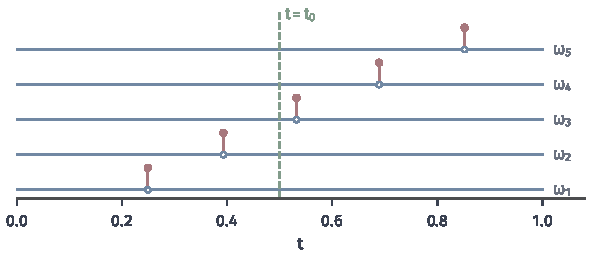
\includegraphics[width=100mm]{figures/03-optimization-evolution-and-signals/02-processes-and-trajectory-evolution/matplotlib/spp-spike/figure.pdf}
  \caption{随机位置的尖点$X_t=\mathbb I_{\{t=U\}}$，$U\sim\mathrm{Unif}(0,1)$。五行是五次独立实现（固定随机种子，纵向错开排列），每行蓝线取值$0$，红点为$t=U$处的取值$1$，空心点表示该处不取$0$。绿色虚线固定时刻$t_0=0.5$：在任何固定时刻，几乎所有实现都取$0$，与零过程无法区分；但每条路径都不连续。}
  \label{fig:spp-spike}
\end{figure}

这个例子直接回答了上一节末尾的问题：$X$与$Y$有相同的有限维分布，一个路径处处连续，一个路径处处有间断。所以有限维分布不能决定路径是否连续，“由有限维分布构造出的过程是否连续”这个问题本身就不恰当；恰当的问题是“它是否有一个连续的版本”。

索引可数时不会出现这种分歧：若$T$可数且$Y$是$X$的版本，则$N=\bigcup_{t\in T}\{X_t\ne Y_t\}$是可数个零概率事件的并，仍为零概率事件，$X$与$Y$不可区分。离散时间过程因此不必区分这两种相等。

\paragraph{右连续版本的比较}
连续时间中，路径正则性可以让可数个时刻代替全部时刻。

\begin{theorem}[右连续版本的唯一性]
\label{thm:spp-right-continuous-versions}
设$T=[0,\infty)$，过程$X,Y$取值于$\mathbb R^d$，$Y$是$X$的版本，并且存在零概率事件$N_0$，使$\omega\notin N_0$时$X$与$Y$的路径都右连续。则$X$与$Y$不可区分。
\end{theorem}

\begin{proof}
令$\mathbb Q_+=\mathbb Q\cap[0,\infty)$，$N=N_0\cup\bigcup_{q\in\mathbb Q_+}\{X_q\ne Y_q\}$。这是可数个零概率事件的并，$\mathbb P(N)=0$。对$\omega\notin N$与任意$t\ge0$，取有理数$q_k\downarrow t$，由右连续性
\[
  X_t(\omega)=\lim_{k\to\infty}X_{q_k}(\omega)=\lim_{k\to\infty}Y_{q_k}(\omega)=Y_t(\omega).
\]
所以在$N$之外两条路径处处相等。
\end{proof}

尖点例子中$X$的路径在$U$处不是右连续的（取值$1$，右侧紧邻处取$0$），所以与定理不矛盾。定理的一个直接推论是：一个过程若有连续版本，这个连续版本在不可区分的意义下唯一。于是，说“过程$X$的连续版本具有某种路径性质”是有确切含义的。

\paragraph{Hölder连续性}
在给出连续版本的判据之前，先约定一种刻画路径粗糙程度的尺度。设$0<\gamma\le1$，函数$x:[0,1]\to\mathbb R^d$若存在常数$C$使
\[
  |x(t)-x(s)|\le C|t-s|^\gamma,\qquad s,t\in[0,1],
\]
就称$x$是$\gamma$阶\term{Hölder连续}（Hölder continuous）的。$\gamma=1$是Lipschitz条件；$\gamma$越小，允许的短程变化越剧烈。例如$\sqrt t$满足$|\sqrt t-\sqrt s|\le|t-s|^{1/2}$，却在零点附近斜率无界，不是Lipschitz的。想象把路径的一小段放大：若时间放大$2$倍，高度最多放大$2^\gamma$倍。对随机路径，常数$C$可以依赖具体的实现$\omega$。

\paragraph{Kolmogorov连续性准则}
要找连续版本，需要同时控制所有短时间增量。下面的准则只要求一个关于增量矩的不等式，就能给出连续版本，并且附带Hölder指数。

\begin{theorem}[Kolmogorov连续性准则]
\label{thm:spp-kolmogorov-continuity}
设$X=(X_t)_{t\in[0,1]}$取值于$\mathbb R^d$。若存在常数$p>0$、$\beta>0$、$C<\infty$，使
\begin{equation}
  \mathbb E|X_t-X_s|^p\le C|t-s|^{1+\beta},\qquad s,t\in[0,1],
  \label{eq:spp-kolmogorov-moment}
\end{equation}
则$X$有一个路径连续的版本$\tilde X$；并且对每个$\gamma\in(0,\beta/p)$，$\tilde X$的几乎所有路径都是$\gamma$阶Hölder连续的。
\end{theorem}

这一结论称为\term{Kolmogorov连续性准则}（Kolmogorov continuity criterion）。证明的想法是先在二进有理点上逐层控制相邻点的增量，再把一般两点之间的增量拆成每层至多一步的链。证明用到Markov不等式和Borel--Cantelli引理：若一列事件的概率之和有限，则几乎必然只有有限个事件发生；它们可参考\BookChapterRef{chap:random-variable-convergence}{卷二“随机变量的收敛与积分极限”章}。

\begin{proof}
固定$\gamma\in(0,\beta/p)$。记第$n$层二进点为$D_n=\{k2^{-n}:\ k=0,1,\ldots,2^n\}$，$D=\bigcup_nD_n$。

第一步，逐层控制相邻增量。令$A_n$为事件“存在$k$使$|X_{k2^{-n}}-X_{(k-1)2^{-n}}|\ge2^{-\gamma n}$”。对每个$k$用Markov不等式和条件\eqref{eq:spp-kolmogorov-moment}，再对$2^n$个$k$求和：
\[
  \mathbb P(A_n)\le2^n\cdot\frac{C\,2^{-n(1+\beta)}}{2^{-\gamma np}}=C\,2^{-n(\beta-\gamma p)} .
\]
由$\gamma p<\beta$，右边对$n$求和有限。由Borel--Cantelli引理，存在零概率事件$N$，使对$\omega\notin N$有整数$n_0(\omega)$，当$n\ge n_0(\omega)$时第$n$层所有相邻增量都小于$2^{-\gamma n}$。

第二步，把一般二进点之间的增量拆成链。固定$\omega\notin N$和$m\ge n_0(\omega)$。对$t\in D$，记$t_m=\lfloor2^mt\rfloor2^{-m}$为$t$在第$m$层左侧最近的点。$t$与$t_m$之间可以用一条链连接：从$t_m$出发，在第$m+1,m+2,\ldots$层各至多走一步相邻点，有限步后到达$t$。每一步的增量小于该层的$2^{-\gamma n}$，因此
\[
  |X_t-X_{t_m}|\le\sum_{n>m}2^{-\gamma n}=\frac{2^{-\gamma(m+1)}}{1-2^{-\gamma}} .
\]
若$s,t\in D$且$|t-s|\le2^{-m}$，则$s_m,t_m$相同或在第$m$层相邻，$|X_{t_m}-X_{s_m}|<2^{-\gamma m}$。三段相加得
\[
  |X_t-X_s|\le c_\gamma\,2^{-\gamma m},\qquad c_\gamma=1+\frac{2\cdot2^{-\gamma}}{1-2^{-\gamma}} .
\]
对$s,t\in D$，$0<|t-s|\le2^{-n_0}$，取$m\ge n_0$使$2^{-m-1}<|t-s|\le2^{-m}$，就得到$|X_t-X_s|\le c_\gamma2^\gamma|t-s|^\gamma$。距离大于$2^{-n_0}$的两点可以用不超过$2^{n_0}$段短距离的链连接，所以$X$限制在$D$上是$\gamma$阶Hölder连续的，常数依赖$\omega$。

第三步，延拓并验证是版本。对$\omega\notin N$，$X_\cdot(\omega)$在稠密集$D$上一致连续，因而对每个$t\in[0,1]$，极限$\tilde X_t(\omega)=\lim_{s\to t,\,s\in D}X_s(\omega)$存在，所得函数$\tilde X_\cdot(\omega)$连续，并保持同样的Hölder估计；对$\omega\in N$令$\tilde X_t(\omega)=0$。每个$\tilde X_t$是可测函数的逐点极限，因而可测。最后固定$t$，取$s_k\in D$，$s_k\to t$。由条件\eqref{eq:spp-kolmogorov-moment}和Markov不等式，$\mathbb P(|X_{s_k}-X_t|>\delta)\le C|s_k-t|^{1+\beta}/\delta^p\to0$，即$X_{s_k}$依概率收敛到$X_t$；同时$X_{s_k}$几乎必然收敛到$\tilde X_t$。依概率收敛的极限几乎必然唯一，所以$\tilde X_t=X_t$几乎必然成立。

上面对固定的$\gamma$证明了Hölder性。取一列$\gamma_j\uparrow\beta/p$，对每个$\gamma_j$得到一个零概率例外事件，它们的并仍是零概率事件；由于连续版本在不可区分意义下唯一，这些$\tilde X$可以取为同一个过程。
\end{proof}

指数中的“$1+\beta$”不能换成$1$。图~\ref{fig:spp-increment-moments}比较了两个过程的增量矩。对Brownian运动，增量$B_{t+h}-B_t\sim\mathcal N(0,h)$，二阶矩为$h$，四阶矩为$3h^2$；取$p=4$、$\beta=1$，准则给出连续版本，且路径是任意$\gamma<1/4$阶Hölder连续的。更一般地，高斯变量的$2r$阶矩为$(2r-1)!!\,h^r$，取$p=2r$、$\beta=r-1$，得到任意$\gamma<(r-1)/(2r)$，令$r\to\infty$即任意$\gamma<1/2$。对速率$\lambda$的Poisson计数过程，$N_{t+h}-N_t$取非负整数值，对任意$p>0$都有
\[
  \mathbb E|N_{t+h}-N_t|^p\ge\mathbb P(N_{t+h}-N_t\ge1)=1-e^{-\lambda h},
\]
它在$h\to0$时与$\lambda h$同阶，指数只能是$1$。准则不适用，这与计数路径必然跳跃相一致。图中两条二阶矩曲线几乎重合，说明只看二阶矩无法区分“连续而粗糙”与“偶尔跳跃”；四阶矩的斜率才把两者分开。准则只是充分条件，不满足它的过程也可能有连续版本。

\begin{figure}[htbp]
  \centering
  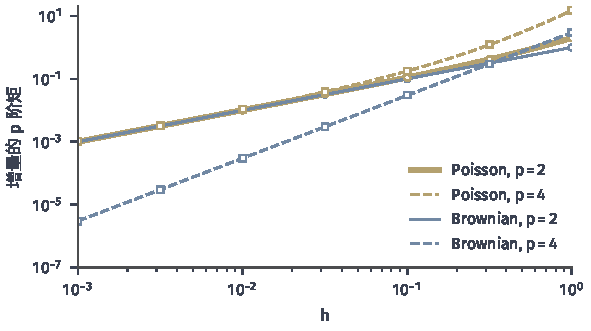
\includegraphics[width=100mm]{figures/03-optimization-evolution-and-signals/02-processes-and-trajectory-evolution/matplotlib/spp-increment-moments/figure.pdf}
  \caption{增量的$p$阶矩$\mathbb E|X_{t+h}-X_t|^p$随时间间隔$h$的变化（双对数坐标）。曲线为精确值：Brownian运动$p=2$为$h$，$p=4$为$3h^2$；速率$1$的Poisson计数过程$p=2$为$h+h^2$，$p=4$为$h+7h^2+6h^3+h^4$。空心点为每个$h$下$200000$次独立抽样的Monte Carlo估计（固定随机种子）。Brownian的四阶矩斜率为$2$，满足Kolmogorov准则；Poisson的各阶矩在小$h$处斜率都是$1$。}
  \label{fig:spp-increment-moments}
\end{figure}

准则陈述在$[0,1]$上，平移和缩放后适用于任何紧区间。对$T=[0,\infty)$，在每个$[k,k+1]$上分别取连续版本；相邻两段在公共端点$k+1$处都几乎必然等于$X_{k+1}$，把它们拼接起来，除一个零概率事件外得到整个半轴上的连续版本。

\paragraph{路径性质与路径极限}
本小节的结论为第~\ref{chap:continuous-time-stochastic-processes}章准备了两件事。第一，Brownian运动由独立高斯增量规定有限维分布，经扩张定理得到坐标过程，再由上面的四阶矩计算取连续版本；那里将据此研究Brownian路径的性质。第二，许多连续时间模型是离散模型在步长趋零时的极限，例如缩放后的随机游走。对一列过程，每个过程分别有连续版本并不够；要得到路径层面的极限，还需要对整列过程统一地控制增量，这一条件及相应的极限定理也在那一章建立。

% 第4章第4节：高斯过程（均值与协方差、半正定性、样本路径与核空间）。

\section{高斯过程}
\label{sec:spp-gaussian-processes}

Kolmogorov扩张定理把构造过程归结为写下一族相容的有限维分布。高斯分布是最容易写全的一族：只要给出均值和协方差，任意有限个位置上的联合分布就确定了，并且删去坐标后的边缘仍是高斯分布。本节利用这一点，在任意索引集上构造随机函数，索引可以是时间，也可以是空间位置或一般输入。我们先说明均值函数与协方差函数怎样确定过程、协方差需要满足什么条件，再讨论样本路径的正则性，并把协方差作为随机函数的规律与它作为再生核所定义的确定性函数空间区分开来。由观测推断未知函数的高斯过程回归不在本节讨论。

\subsection{均值、协方差与联合高斯规律}
\label{sec:spp-gp-definition}

\paragraph{允许奇异协方差的高斯向量}
有限维高斯分布通常用密度定义，这要求协方差矩阵正定。构造过程时却经常遇到奇异的协方差：例如三个位置上的读数可能由两个随机系数完全决定。下面采用不依赖密度的说法。随机向量$\bm Y\in\mathbb R^m$称为高斯向量，若存在$\bm\mu\in\mathbb R^m$、矩阵$\bm A\in\mathbb R^{m\times r}$和由独立标准高斯变量组成的$\bm Z\in\mathbb R^r$，使$\bm Y=\bm\mu+\bm A\bm Z$。此时$\mathbb E\bm Y=\bm\mu$，$\operatorname{Cov}(\bm Y)=\bm A\bm A^\top$。

这个定义有三条性质需要用到。第一，任意对称半正定矩阵$\bm\Sigma$都可以作为协方差：取谱分解$\bm\Sigma=\bm Q\bm\Lambda\bm Q^\top$，令$\bm A=\bm Q\bm\Lambda^{1/2}$即可。第二，分布只依赖$(\bm\mu,\bm\Sigma)$：$\bm Y$的特征函数为$\mathbb E e^{\mathrm i\bm c^\top\bm Y}=\exp(\mathrm i\bm c^\top\bm\mu-\tfrac12\bm c^\top\bm\Sigma\bm c)$，而特征函数决定分布；记作$\bm Y\sim\mathcal N(\bm\mu,\bm\Sigma)$。第三，线性像仍是高斯向量：对矩阵$\bm B$，$\bm B\bm Y=\bm B\bm\mu+(\bm B\bm A)\bm Z$，所以$\bm B\bm Y\sim\mathcal N(\bm B\bm\mu,\bm B\bm\Sigma\bm B^\top)$。$\bm\Sigma$正定时，这与用密度定义的\term{多元高斯分布}（multivariate Gaussian distribution）一致，后者及其仿射变换性质可参考\BookChapterRef{chap:random-vectors}{卷一“随机向量与联合分布”章}；$\bm\Sigma$奇异时，$\bm Y$集中在一个仿射子空间上，没有密度。

\paragraph{高斯过程的定义}
把“任意有限个读数联合高斯”作为定义，就得到高斯过程。

\begin{definition}[高斯过程]
\label{def:spp-gaussian-process}
实值随机过程$F=(F(x))_{x\in\mathcal X}$称为\term{高斯过程}（Gaussian process），若对任意正整数$m$和任意$x_1,\ldots,x_m\in\mathcal X$，随机向量$(F(x_1),\ldots,F(x_m))^\top$都是高斯向量。函数
\[
  m(x)=\mathbb EF(x),\qquad k(x,x')=\operatorname{Cov}\bigl(F(x),F(x')\bigr)
\]
分别称为它的\term{均值函数}（mean function）与\term{协方差函数}（covariance function），记作$F\sim\mathcal{GP}(m,k)$。
\end{definition}

索引集$\mathcal X$可以是任意集合，不需要顺序，也不需要拓扑。由第三条性质，$(F(x_1),\ldots,F(x_m))^\top$的分布是均值为$(m(x_i))_i$、协方差为$(k(x_i,x_j))_{i,j}$的高斯分布，所以$m$与$k$决定了全部有限维分布，从而决定了路径规律。

定义中“联合”二字不可省略。设$X\sim\mathcal N(0,1)$，符号$S$与$X$独立、等概率取$\pm1$。则$X$与$SX$都服从$\mathcal N(0,1)$，且$\operatorname{Cov}(X,SX)=\mathbb ES\cdot\mathbb EX^2=0$。但$X+SX$以概率$1/2$恰好为$0$，以概率$1/2$等于$2X$，它不是高斯变量；所以$(X,SX)$不是高斯向量，尽管两个坐标各自高斯且不相关。逐点高斯并不足以构成高斯过程。

\paragraph{存在性：半正定是充要条件}
哪些函数$k$可以作为协方差函数？答案是半正定性，它既是必要的，也是充分的。

\begin{theorem}[高斯过程的存在与唯一]
\label{thm:spp-gp-existence}
设$\mathcal X$是非空集合，$m:\mathcal X\to\mathbb R$，$k:\mathcal X\times\mathcal X\to\mathbb R$。存在以$m$为均值函数、$k$为协方差函数的高斯过程，当且仅当$k$对称，并且对任意有限个$x_1,\ldots,x_n\in\mathcal X$和实数$c_1,\ldots,c_n$都有
\begin{equation}
  \sum_{i,j=1}^nc_ic_j\,k(x_i,x_j)\ge0 .
  \label{eq:spp-psd}
\end{equation}
满足这一条件时，过程在$(\mathbb R^{\mathcal X},\mathcal B(\mathbb R)^{\otimes\mathcal X})$上的路径规律唯一。
\end{theorem}

\begin{proof}
必要性：若过程存在，协方差由
\[
  \operatorname{Cov}(F(x),F(x'))=\operatorname{Cov}(F(x'),F(x))
\]
对称，并且$\sum_{i,j}c_ic_jk(x_i,x_j)=\operatorname{Var}\bigl(\sum_ic_iF(x_i)\bigr)\ge0$。这一步只用到二阶矩，所以任何二阶矩有限的过程的协方差函数都满足式~\eqref{eq:spp-psd}。

充分性：对有限集$J\subseteq\mathcal X$，矩阵$\bm K_J=(k(s,t))_{s,t\in J}$对称且由式~\eqref{eq:spp-psd}半正定，令$\mu_J=\mathcal N\bigl((m(t))_{t\in J},\bm K_J\bigr)$。对有限集$J\subseteq K$，限制映射$\pi_{K,J}$是删去坐标的线性映射，由线性像的性质，$\mu_K\circ\pi_{K,J}^{-1}$是均值为$(m(t))_{t\in J}$、协方差为$\bm K_K$的子矩阵$\bm K_J$的高斯分布，即$\mu_J$。所以这一族相容。$\mathbb R$是标准Borel空间，由定理~\ref{thm:spp-kolmogorov-extension}得到所需过程。唯一性来自有限维分布由$(m,k)$决定以及定理~\ref{thm:spp-path-law}。
\end{proof}

满足式~\eqref{eq:spp-psd}的对称函数称为\term{半正定}（positive semidefinite）核。定理把“构造一个高斯过程”化为“检查一个二元函数半正定”，后者是纯粹的确定性问题。

\paragraph{几种协方差结构}
下面几类协方差依次说明，核怎样规定读数之间的依赖，以及怎样检查半正定性。

\emph{常数核。}$k(x,x')\equiv\sigma^2$。取$Z\sim\mathcal N(0,1)$，令$F(x)=\sigma Z$对一切$x$成立，即得此过程：所有位置读数相同，整条路径是一条随机高度的水平线。任意$n$个位置的协方差矩阵秩为$1$。

\emph{有限随机基展开。}取确定函数$\varphi_1,\ldots,\varphi_r$和独立标准高斯变量$Z_1,\ldots,Z_r$，令$F(x)=\sum_{j=1}^rZ_j\varphi_j(x)$。则$k(x,x')=\sum_j\varphi_j(x)\varphi_j(x')$，半正定性自动成立：$\sum_{i,l}c_ic_lk(x_i,x_l)=\sum_j\bigl(\sum_ic_i\varphi_j(x_i)\bigr)^2\ge0$。任意多个位置上的读数都由$r$个系数决定，协方差矩阵的秩至多为$r$。例如$F(x)=A+Bx$，$A,B$独立标准高斯，$k(x,x')=1+xx'$；在$x=0,1,2$处
\[
  \bm K=\begin{pmatrix}1&1&1\\1&2&3\\1&3&5\end{pmatrix},\qquad \det\bm K=0,
\]
因为三个读数满足$F(0)-2F(1)+F(2)=0$。

\emph{平稳核。}在$\mathcal X=\mathbb R$上，若$k(x,x')=\kappa(x-x')$只依赖位置差，则读数的依赖不随整体平移改变。常用的有\term{平方指数核}（squared exponential kernel）$\kappa(h)=\sigma^2e^{-h^2/(2\ell^2)}$和\term{指数核}（exponential kernel）$\kappa(h)=\sigma^2e^{-|h|/\ell}$，长度尺度$\ell$控制相关性衰减的距离。检查它们半正定有一个统一的办法：若$\kappa(h)=\sigma^2\,\mathbb Ee^{\mathrm iWh}$是某个对称分布$W$的特征函数乘以$\sigma^2$，则
\[
  \sum_{i,j}c_ic_j\kappa(x_i-x_j)=\sigma^2\,\mathbb E\Bigl|\sum_jc_je^{\mathrm iWx_j}\Bigr|^2\ge0 .
\]
$e^{-h^2/(2\ell^2)}$是$\mathcal N(0,\ell^{-2})$的特征函数，$e^{-|h|/\ell}$是密度为$\ell/\bigl(\pi(1+\ell^2w^2)\bigr)$的Cauchy分布的特征函数，所以两者都半正定。\term{周期核}（periodic kernel）$k(x,x')=\sigma^2\exp\bigl(-2\sin^2(\pi(x-x')/p)/\ell^2\bigr)$可以化归为平方指数核：令$\bm u(x)=(\cos(2\pi x/p),\sin(2\pi x/p))$，则$|\bm u(x)-\bm u(x')|^2=4\sin^2(\pi(x-x')/p)$，周期核就是平面$\mathbb R^2$上的平方指数核在点$\bm u(x_1),\ldots,\bm u(x_n)$处的取值。平方指数核在$\mathbb R^2$上的半正定性同样来自二元高斯分布的特征函数。

\emph{Brownian核。}在$\mathcal X=[0,\infty)$上，$k(s,t)=\min(s,t)$也称\term{最小值核}（minimum kernel）。它半正定，因为
\[
  \sum_{i,j}c_ic_j\min(t_i,t_j)=\int_0^\infty\Bigl(\sum_ic_i\mathbb I_{\{u\le t_i\}}\Bigr)^2\mathrm du\ge0 ,
\]
这里用了$\int_0^\infty\mathbb I_{\{u\le t_i\}}\mathbb I_{\{u\le t_j\}}\,\mathrm du=\min(t_i,t_j)$。均值为零、协方差为$\min(s,t)$的高斯过程就是Brownian运动的有限维规律：对$s<t$，$\operatorname{Var}(F(t)-F(s))=t-2s+s=t-s$，不相交区间上的增量不相关因而独立。

并非每个看起来合理的“相似度”都半正定。取$k(x,x')=\mathbb I_{\{|x-x'|\le1\}}$，即距离不超过$1$的两点完全相关、否则不相关。在$x=0,0.75,1.5$处，系数$c=(1,-1,1)$给出
\[
  \sum_{i,j}c_ic_jk(x_i,x_j)=3-2\cdot1-2\cdot1+2\cdot0=-1<0 ,
\]
所以不存在以它为协方差的过程。

图~\ref{fig:spp-gp-kernels}把四个核的协方差矩阵画成热图，并在每个核下抽取三条样本路径。对角线附近的颜色宽度对应相关距离：平方指数核的路径光滑，指数核的路径粗糙，周期核的路径以$p=0.5$为周期重复，Brownian核的路径从$0$出发、方差随$t$增长。前三个核在每个位置的方差都是$1$，路径外观的差别完全来自位置之间的相关结构；Brownian核的方差$t$则随位置增长。

\begin{figure*}[htbp]
  \centering
  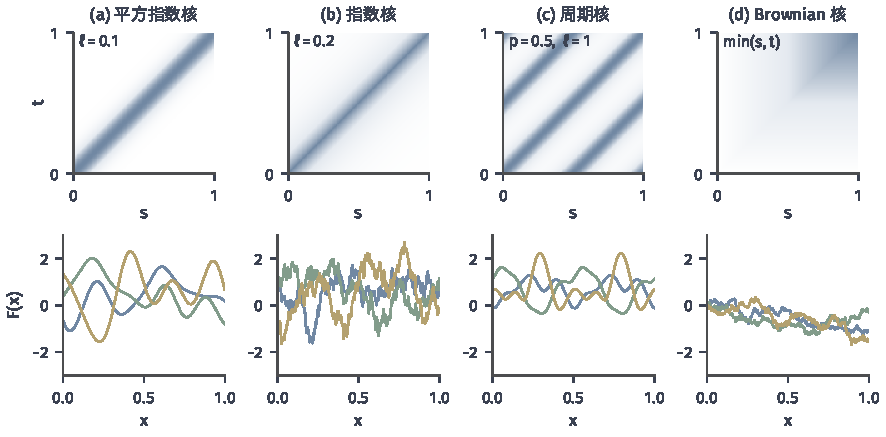
\includegraphics[width=150mm]{figures/03-optimization-evolution-and-signals/02-processes-and-trajectory-evolution/matplotlib/spp-gp-kernels/figure.pdf}
  \caption{四种协方差函数及相应高斯过程的样本路径，定义域$[0,1]$，$\sigma^2=1$。上排为$k(s,t)$在$301\times301$网格上的热图（白色为$0$，蓝色为$1$）；下排为对应的三条样本路径，用网格协方差矩阵的特征分解抽样（固定随机种子，三条路径在四个核下使用同一组标准高斯向量）。(a)平方指数核，$\ell=0.1$；(b)指数核，$\ell=0.2$；(c)周期核，$p=0.5$，$\ell=1$；(d)Brownian核$\min(s,t)$。}
  \label{fig:spp-gp-kernels}
\end{figure*}

索引不必是一维时间。在平面区域上取$k(\bm x,\bm x')=\sigma^2e^{-|\bm x-\bm x'|^2/(2\ell^2)}$，得到的随机场在距离小于$\ell$的位置上读数相近，可用来描述一片区域上的气温偏差；这里没有“过去”和“将来”，逐步构造无从谈起，扩张定理却照样适用。

\paragraph{在有限网格上抽样}
计算机只能在有限个位置上抽样。给定网格$x_1,\ldots,x_n$，计算矩阵$\bm K=(k(x_i,x_j))_{i,j}$，求一个分解$\bm K=\bm A\bm A^\top$，再令$(F(x_i))_i=(m(x_i))_i+\bm A\bm Z$，其中$\bm Z$是$n$维标准高斯向量。$\bm K$正定时常用Cholesky分解，计算量为$O(n^3)$，存储为$O(n^2)$；$\bm K$奇异或接近奇异时（例如平方指数核在密集网格上），可以用特征分解并把舍入误差造成的微小负特征值截为零，图~\ref{fig:spp-gp-kernels}就是这样生成的。实践中也常在对角线上加一个小量$\epsilon$再做Cholesky分解；这相当于给每个读数加上独立的$\mathcal N(0,\epsilon)$噪声，抽到的是略有不同的过程，$\epsilon$应当相对于核的尺度足够小。

\paragraph{有限基展开逼近Brownian运动}
有限随机基展开不仅是一个例子，也是构造一般高斯过程的方法。对Brownian核，令$a_k=(k-\tfrac12)\pi$，$e_k(t)=\sqrt2\sin(a_kt)/a_k$，$k\ge1$。对$s,t\in[0,1]$有恒等式
\begin{equation}
  \min(s,t)=\sum_{k=1}^\infty e_k(s)e_k(t) .
  \label{eq:spp-min-expansion}
\end{equation}
验证如下：$\{\sqrt2\sin(a_kt)\}_{k\ge1}$是$L^2[0,1]$的标准正交基；固定$s$，函数$t\mapsto\min(s,t)$在这组基下的系数为
\[
  \begin{aligned}
  \sqrt2\int_0^1\min(s,t)\sin(a_kt)\,\mathrm dt
  &=\sqrt2\Bigl(\int_0^st\sin(a_kt)\,\mathrm dt+s\int_s^1\sin(a_kt)\,\mathrm dt\Bigr)\\
  &=\frac{\sqrt2\sin(a_ks)}{a_k^2},
  \end{aligned}
\]
其中分部积分后用了$\cos a_k=0$。于是$\min(s,\cdot)=\sum_k\frac{\sqrt2\sin(a_ks)}{a_k^2}\sqrt2\sin(a_k\cdot)$在$L^2$意义下成立；右边的级数被$\sum_k2/a_k^2<\infty$一致控制，因而绝对一致收敛到一个连续函数，它与连续函数$\min(s,\cdot)$几乎处处相等，故处处相等。

取独立标准高斯变量$Z_1,Z_2,\ldots$，令$W^{(m)}(t)=\sum_{k=1}^mZ_ke_k(t)$。每个$W^{(m)}$是有限基展开的高斯过程，协方差为式~\eqref{eq:spp-min-expansion}的前$m$项部分和。对固定的$t$，各项独立、均值为零，方差之和$\sum_ke_k(t)^2=t$有限，所以级数几乎必然且在$L^2$中收敛；极限$W(t)$是高斯变量，协方差由式~\eqref{eq:spp-min-expansion}给出$\min(s,t)$。图~\ref{fig:spp-kl-expansion}用同一组系数画出$m=1,4,16,1024$时的部分和：项数少时路径光滑，每加入一组高频项就添上更细的起伏，逐渐接近Brownian路径的粗糙外形。这类按协方差的特征函数展开的表示称为\term{Karhunen--Loève展开}（Karhunen--Loève expansion）。

\begin{figure}[htbp]
  \centering
  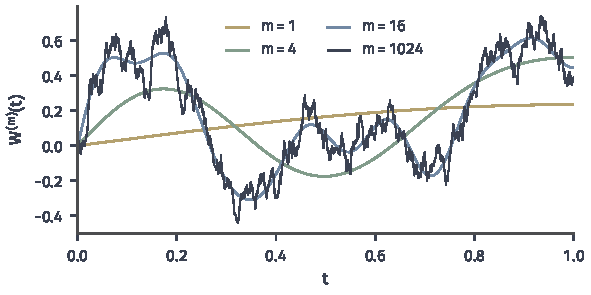
\includegraphics[width=100mm]{figures/03-optimization-evolution-and-signals/02-processes-and-trajectory-evolution/matplotlib/spp-kl-expansion/figure.pdf}
  \caption{Brownian运动的有限基展开$W^{(m)}(t)=\sum_{k\le m}Z_k\sqrt2\sin\bigl((k-\tfrac12)\pi t\bigr)/\bigl((k-\tfrac12)\pi\bigr)$。四条曲线使用同一组独立标准高斯系数$Z_1,Z_2,\ldots$（固定随机种子），仅截断项数$m=1,4,16,1024$不同。每条部分和都是光滑函数，随项数增加逐步出现更细的起伏。}
  \label{fig:spp-kl-expansion}
\end{figure}

\subsection{样本路径与核空间的区别}
\label{sec:spp-gp-paths-rkhs}

\paragraph{增量方差控制路径}
高斯过程的路径性质由协方差决定，具体地说由增量方差决定。设$F\sim\mathcal{GP}(0,k)$，令
\[
  d^2(s,t)=\mathbb E\bigl(F(t)-F(s)\bigr)^2=k(t,t)-2k(s,t)+k(s,s).
\]
增量$F(t)-F(s)\sim\mathcal N(0,d^2(s,t))$，它的高阶矩完全由$d$决定：$\mathbb E|F(t)-F(s)|^{2r}=(2r-1)!!\,d(s,t)^{2r}$。于是只要$d^2$随间隔以幂次衰减，就可以选足够高的矩阶使用Kolmogorov连续性准则。

\begin{theorem}[高斯过程的连续版本]
\label{thm:spp-gp-continuity}
设$F\sim\mathcal{GP}(0,k)$，索引集为$[0,1]$。若存在$C<\infty$与$\alpha>0$使
\[
  d^2(s,t)\le C|t-s|^\alpha,\qquad s,t\in[0,1],
\]
则$F$有连续版本，并且对每个$\gamma\in(0,\alpha/2)$，其几乎所有路径都是$\gamma$阶Hölder连续的。
\end{theorem}

\begin{proof}
取正整数$r$使$r\alpha>1$。则$\mathbb E|F(t)-F(s)|^{2r}\le(2r-1)!!\,C^r|t-s|^{r\alpha}$，满足定理~\ref{thm:spp-kolmogorov-continuity}的条件，其中$p=2r$，$\beta=r\alpha-1$。所得Hölder指数可以取任意小于$\beta/p=\alpha/2-1/(2r)$的值；$r$可以任意大，于是对任意$\gamma<\alpha/2$都成立。
\end{proof}

对Brownian核，$d^2(s,t)=|t-s|$，$\alpha=1$，路径是任意$\gamma<1/2$阶Hölder连续的，这与第~\ref{sec:spp-versions}小节的直接计算一致。对指数核，$d^2(s,t)=2\sigma^2(1-e^{-|t-s|/\ell})\le2\sigma^2|t-s|/\ell$，同样$\alpha=1$：它的路径与Brownian路径一样粗糙，这正是图~\ref{fig:spp-gp-kernels}(b)中看到的。对平方指数核，$1-e^{-u}\le u$给出$d^2(s,t)\le\sigma^2|t-s|^2/\ell^2$，$\alpha=2$，定理给出任意$\gamma<1$阶Hölder连续；它的路径实际上更光滑（任意阶可微），这需要对导数过程再做类似的估计，此处不展开。

\paragraph{均方连续不等于路径连续}
若$d(s,t)\to0$（$s\to t$），称过程\term{均方连续}（mean-square continuous）。这只说明每个固定时刻附近的增量在平均意义上很小，并不控制所有时刻同时发生的事。速率$\lambda$的Poisson计数过程是一个非高斯的例子：$\mathbb E(N_t-N_s)^2=\lambda h+\lambda^2h^2\to0$，它均方连续，而几乎每条路径都有跳跃。对高斯过程，均方连续同样不足以保证连续版本：增量标准差趋于零的速度若太慢，例如只像$(\log(1/h))^{-1/2}$那样衰减，可以构造出在每个区间上几乎必然无界的平稳高斯过程。关于高斯过程路径连续的精确判据涉及度量熵，本书不展开；定理~\ref{thm:spp-gp-continuity}的幂次条件是实践中最常用的充分条件。

\paragraph{同一个核的两种用途}
半正定核在函数空间部分以另一种身份出现过：每个半正定核$k$唯一确定一个由$\mathcal X$上函数组成的Hilbert空间$H_k$，称为\term{再生核Hilbert空间}（reproducing kernel Hilbert space），其中$k(\cdot,x)\in H_k$，并且对每个$f\in H_k$有再生性质$\langle f,k(\cdot,x)\rangle_{H_k}=f(x)$；可参考\BookChapterRef{chap:rkhs}{卷二“再生核Hilbert空间”章}。于是同一个$k$有两种用途：作为协方差，它规定一个随机函数的规律；作为再生核，它规定一个确定性的函数空间及其范数。两者很容易被混为一谈，以为高斯过程的样本就是$H_k$中的随机元素。

有限维情形下这样想是对的。设$F=\sum_{j=1}^rZ_j\varphi_j$，$\varphi_1,\ldots,\varphi_r$线性无关，则$k=\sum_j\varphi_j\otimes\varphi_j$，$H_k$就是$\operatorname{span}\{\varphi_1,\ldots,\varphi_r\}$，并且$\bigl\|\sum_ja_j\varphi_j\bigr\|_{H_k}^2=\sum_ja_j^2$。每个样本$F$都落在$H_k$中，范数平方$\|F\|_{H_k}^2=\sum_{j\le r}Z_j^2$的期望为$r$。这个期望随维数增长：基越多，样本在$H_k$范数下越“大”。无限维时，这一增长会使样本完全离开$H_k$。

\paragraph{Brownian路径不在核空间中}
以Brownian核为例说明。函数空间部分已经算出，$[0,1]$上最小值核的再生核Hilbert空间是
\begin{gather*}
  H_{\min}=\Bigl\{f:[0,1]\to\mathbb R:\ f(0)=0,\ f\text{绝对连续},\ f'\in L^2[0,1]\Bigr\},\\
  \|f\|_{H_{\min}}^2=\int_0^1f'(t)^2\,\mathrm dt .
\end{gather*}
展开式~\eqref{eq:spp-min-expansion}中的$e_k$满足$e_k'(t)=\sqrt2\cos(a_kt)$，它们在$H_{\min}$中标准正交，所以部分和$W^{(m)}$在$H_{\min}$中的范数平方是$\sum_{k\le m}Z_k^2$。由强大数律，它几乎必然像$m$一样增长到无穷，图~\ref{fig:spp-rkhs-vs-path}(b)显示了三组系数下的这一增长。这提示极限$W$不在$H_{\min}$中，下面的定理给出直接的证明。

\begin{theorem}[Brownian路径几乎必然不属于$H_{\min}$]
\label{thm:spp-brownian-not-in-rkhs}
设$W$是$[0,1]$上均值为零、协方差为$\min(s,t)$的高斯过程的连续版本。则$\mathbb P(W\in H_{\min})=0$。
\end{theorem}

\begin{proof}
对函数$f$与$n\ge1$，记二进平方增量和$Q_n(f)=\sum_{i=1}^{2^n}\bigl(f(i2^{-n})-f((i-1)2^{-n})\bigr)^2$。

若$f\in H_{\min}$，在每个长为$2^{-n}$的小区间$I_i$上由Cauchy--Schwarz不等式，
\[
  \bigl(f(i2^{-n})-f((i-1)2^{-n})\bigr)^2=\Bigl(\int_{I_i}f'\Bigr)^2\le2^{-n}\int_{I_i}f'^2 ,
\]
求和得$Q_n(f)\le2^{-n}\|f\|_{H_{\min}}^2\to0$。

对$W$，$Q_n(W)$是$2^n$个独立$\mathcal N(0,2^{-n})$变量的平方和，$\mathbb EQ_n(W)=1$，$\operatorname{Var}Q_n(W)=2^n\cdot2\cdot2^{-2n}=2^{1-n}$。由Chebyshev不等式，$\mathbb P(|Q_n(W)-1|>\tfrac12)\le4\cdot2^{1-n}$，对$n$求和有限；由Borel--Cantelli引理，几乎必然只有有限个$n$使$|Q_n(W)-1|>\tfrac12$，所以几乎必然$Q_n(W)\not\to0$。与上一段对照，几乎必然$W\notin H_{\min}$。
\end{proof}

图~\ref{fig:spp-rkhs-vs-path}(a)直观地展示了这个证明：光滑函数$f(t)=0.8\sin(\pi t/2)\in H_{\min}$的二进平方增量和每细分一层大约减半，紧贴上界$\|f\|^2_{H_{\min}}2^{-n}$；Brownian路径的平方增量和则稳定在$1$附近，不随细分消失。这个量称为二次变差，它在第~\ref{chap:continuous-time-stochastic-processes}章的随机积分中起核心作用。

\begin{figure}[htbp]
  \centering
  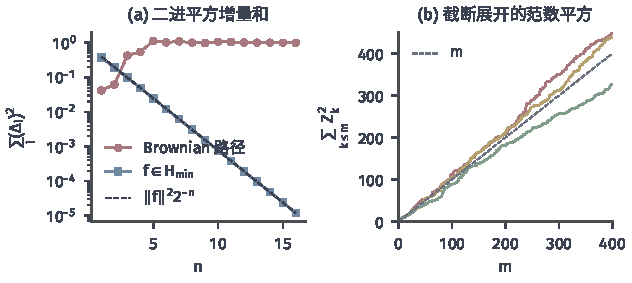
\includegraphics[width=107mm]{figures/03-optimization-evolution-and-signals/02-processes-and-trajectory-evolution/matplotlib/spp-rkhs-vs-path/figure.pdf}
  \caption{Brownian路径与最小值核空间$H_{\min}$的比较。(a)二进平方增量和$Q_n=\sum_i(\Delta_i)^2$随层级$n$的变化（对数纵轴）：红线为一条用$2^{16}$个格点模拟的Brownian路径，蓝线为$f(t)=0.8\sin(\pi t/2)\in H_{\min}$，虚线为上界$\|f\|^2_{H_{\min}}2^{-n}$，其中$\|f\|^2_{H_{\min}}=\int_0^1f'(t)^2\,\mathrm dt=0.08\pi^2\approx0.79$。(b)有限基展开$W^{(m)}$在$H_{\min}$中的范数平方$\sum_{k\le m}Z_k^2$随项数$m$的增长，三条曲线对应三组独立系数，虚线为期望值$m$。随机数均使用固定种子。}
  \label{fig:spp-rkhs-vs-path}
\end{figure}

更一般地，在可分Banach空间上的高斯测度理论中可以证明：协方差的再生核Hilbert空间（在那里称为Cameron--Martin空间）只要是无限维的，其测度就为零。所以对无限维的核，“样本路径属于$H_k$”通常不成立，样本比$H_k$中的典型元素粗糙得多。

\paragraph{两种用途的分工}
$H_k$并没有因此与高斯过程无关。它描述的是：把高斯过程的路径整体平移一个确定函数$h$后，新规律何时与原规律相互绝对连续；答案恰好是$h\in H_k$。第~\ref{chap:continuous-time-stochastic-processes}章研究连续路径的换测度时会用到这一事实的Brownian情形。另一方面，高斯过程回归中，给定有限个观测后的后验均值是$k(\cdot,x_i)$的有限线性组合，因而属于$H_k$；回归、后验及统计保证由卷四的统计推断部分处理。本节的结论是分工：样本路径的正则性由协方差通过增量方差决定，$H_k$刻画的是确定性函数和平移方向，两者不能互相替代。

% 第4章第5节：交换序列（交换性、与独立和平稳的比较、de Finetti表示）。

\section{交换序列}
\label{sec:spp-exchangeable}

前几节的依赖大多来自时间：下一步依赖过去，相邻读数共享增量。但第~\ref{sec:spp-index-state-space}小节的共享背景读数提示了另一种来源：所有观测共同受一个随机背景影响，彼此之间并没有先后作用。Pólya罐的路径概率只依赖$1$的个数（示例~\ref{ex:spp-polya-path}），也是这种结构的表现。本节研究观测编号重排后联合规律不变的序列。我们先比较交换性与独立、与时间平移不变性各约束什么，再说明无限交换序列总可以写成“先抽随机背景，再条件独立抽样”，并解释这为什么使经验平均趋向一个随机的极限。

\subsection{交换性与共享随机背景}
\label{sec:spp-exchangeability}

\paragraph{共享成功率的抛掷}
设想一批硬币来自同一台冲压机，每枚的正面概率都是同一个未知值。把这个未知值建模为随机变量$\Theta\sim\operatorname{Beta}(2,2)$，给定$\Theta$后，各次抛掷$X_1,X_2,\ldots$独立服从$\operatorname{Bernoulli}(\Theta)$。对任一含$k$个$1$的序列$(x_1,\ldots,x_n)$，先对给定$\Theta$的条件概率求积，再对$\Theta$平均：
\[
  \mathbb P(X_1=x_1,\ldots,X_n=x_n)=\mathbb E\bigl[\Theta^k(1-\Theta)^{n-k}\bigr].
\]
右边只依赖$k$，不依赖$1$出现在哪些位置。这是本节的核心现象：观测之间相关，但没有哪个编号是特殊的。

相关性可以直接算出。$\Theta\sim\operatorname{Beta}(2,2)$的均值为$1/2$，方差为$1/20$。对$i\ne j$，由塔式性质，
\begin{gather*}
  \mathbb P(X_i=X_j=1)=\mathbb E\Theta^2=\frac1{20}+\frac14=0.3,\\
  \operatorname{Cov}(X_i,X_j)=\mathbb E\Theta^2-(\mathbb E\Theta)^2=\operatorname{Var}(\Theta)=\frac1{20}.
\end{gather*}
两次都是正面的概率$0.3$大于独立时的$0.25$：观测到一次正面，使“这批硬币偏向正面”更可信，从而提高了下一次正面的概率。成功次数$S_n=X_1+\cdots+X_n$的方差也随之增大。由条件方差分解，
\[
  \begin{aligned}
  \operatorname{Var}(S_n)&=\mathbb E\operatorname{Var}(S_n\mid\Theta)+\operatorname{Var}\mathbb E(S_n\mid\Theta)\\
  &=n\,\mathbb E[\Theta(1-\Theta)]+n^2\operatorname{Var}(\Theta)=\frac n5+\frac{n^2}{20},
  \end{aligned}
\]
其中$\mathbb E[\Theta(1-\Theta)]=\frac12-0.3=0.2$。$n=10$时为$7$，而独立$\operatorname{Bernoulli}(1/2)$的成功次数方差只有$2.5$。图~\ref{fig:spp-beta-binomial}比较了两种分布：共享成功率时，极端的成功次数明显更常见。

\begin{figure}[htbp]
  \centering
  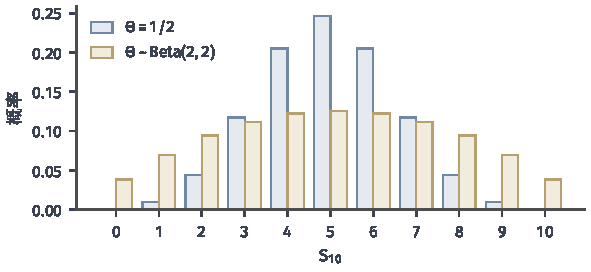
\includegraphics[width=100mm]{figures/03-optimization-evolution-and-signals/02-processes-and-trajectory-evolution/matplotlib/spp-beta-binomial/figure.pdf}
  \caption{十次抛掷中成功次数$S_{10}$的分布（精确概率）。蓝色：成功率固定为$1/2$，各次独立，$S_{10}\sim\operatorname{Bin}(10,1/2)$，方差$2.5$。黄色：成功率$\Theta\sim\operatorname{Beta}(2,2)$由各次共享，给定$\Theta$后独立，方差$7$。两者单次成功概率都是$1/2$。}
  \label{fig:spp-beta-binomial}
\end{figure}

\paragraph{交换性的定义}
把“编号不特殊”写成联合规律的对称性，得到下面的定义。

\begin{definition}[可交换序列]
\label{def:spp-exchangeable}
随机变量$X_1,\ldots,X_n$称为\term{可交换}（exchangeable）的，若对$\{1,\ldots,n\}$的每个排列$\pi$都有
\[
  (X_{\pi(1)},\ldots,X_{\pi(n)})\overset{\mathrm d}{=}(X_1,\ldots,X_n).
\]
无限序列$(X_n)_{n\ge1}$称为可交换的，若对每个$n$，$(X_1,\ldots,X_n)$可交换。这一性质称为\term{交换性}（exchangeability）。
\end{definition}

无限序列的定义等价于：只改变有限个编号的任意排列都不改变整个序列的规律，因为这样的排列只涉及某个前缀，而序列的规律由有限维分布决定。由定义，可交换序列的各项同分布，任意两项的联合分布都相同，任意$m$项的联合分布也只依赖$m$。

\paragraph{交换与独立各约束什么}
交换性与独立性约束联合规律的不同方面。独立同分布序列可交换，因为其联合分布是同一边缘分布的乘积，重排因子不改变乘积。反之，上面的共享成功率序列可交换却不独立；而独立但分布不同的序列，例如$X_i\sim\mathcal N(i,1)$相互独立，则独立却不可交换。独立性说的是联合规律能否分解为乘积，交换性说的是联合规律在重排下是否对称。

交换性对相关系数有一个简单的约束。设$X_1,\ldots,X_n$可交换，方差$\sigma^2>0$，任意两项的相关系数都是$\rho$。则
\[
  0\le\operatorname{Var}\Bigl(\sum_{i=1}^nX_i\Bigr)=n\sigma^2+n(n-1)\rho\sigma^2=n\sigma^2\bigl(1+(n-1)\rho\bigr),
\]
所以$\rho\ge-1/(n-1)$。对无限可交换序列，这对每个$n$都成立，令$n\to\infty$得$\rho\ge0$。负相关只能出现在有限长的可交换序列中。

\begin{example}[不放回抽取]
\label{ex:spp-without-replacement}
罐中有一个$1$球和一个$0$球，不放回地依次摸出，记标号为$X_1,X_2$。$(X_1,X_2)$等概率地取$(1,0)$或$(0,1)$，重排后分布不变，所以可交换。但$\operatorname{Cov}(X_1,X_2)=0-\frac14=-\frac14$，$\operatorname{Var}(X_i)=\frac14$，相关系数为$-1<-\frac12$。由上面的约束，它不能延长为三个可交换变量，更不能延长为无限可交换序列。它也不能写成“先抽$\Theta$、再条件独立抽样”的形式，因为那样得到的任意两项协方差都等于$\operatorname{Var}(\Theta)\ge0$。更一般地，从$N$个球中不放回抽样得到的有限序列可交换，相关系数为$-1/(N-1)$。
\end{example}

\paragraph{交换性与平移不变性}
时间序列中常见的另一种对称性是平移不变性：若对每个$k\ge0$，$(X_{1+k},X_{2+k},\ldots)$与$(X_1,X_2,\ldots)$同分布，就称序列具有\term{严格平稳性}（strict stationarity），简称平稳。无限可交换序列一定平稳：对固定的$n$和$k$，存在$\{1,\ldots,n+k\}$的一个排列把$(1+k,\ldots,n+k)$移到$(1,\ldots,n)$，由交换性，$(X_{1+k},\ldots,X_{n+k})\overset{\mathrm d}{=}(X_1,\ldots,X_n)$，再由有限维分布决定规律即得。

反之不成立。第~\ref{sec:spp-fdd-path-law}小节的平稳自回归序列（$\rho=0.8$）平移不变，但$\operatorname{Corr}(Y_1,Y_2)=0.8$，$\operatorname{Corr}(Y_1,Y_3)=0.64$；若它可交换，交换第$2$、$3$项不改变规律，就应有$(Y_1,Y_2)\overset{\mathrm d}{=}(Y_1,Y_3)$，两个相关系数必须相等。平稳只要求依赖结构不随整体平移改变，允许远近不同的项依赖强弱不同；交换性要求所有项两两地位相同。两种对称性服务于不同的目的：平稳性用于研究长时间平均（第~\ref{chap:discrete-time-stochastic-processes}章的遍历理论），交换性用于描述顺序无关的抽样和由此得到的置换论证。

\subsection{条件独立混合表示}
\label{sec:spp-de-finetti}

\paragraph{频率的极限是随机的}
图~\ref{fig:spp-polya-frequencies}比较了两类序列的累计频率$\bar X_n=S_n/n$。独立的$\operatorname{Bernoulli}(1/2)$序列中，二十条频率曲线都向$1/2$收拢，这是强大数律。Pólya罐（$a=b=1$）的二十条曲线也各自稳定下来，却停在不同的高度；把四千个罐运行两千步，最终频率的直方图几乎是平的。看起来，每个罐在开头几步的偶然结果中“选定”了一个自己的成功率，此后的观测就像以这个成功率独立抽样。

\begin{figure*}[htbp]
  \centering
  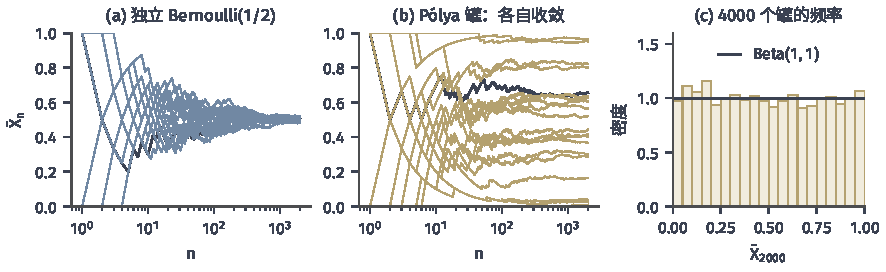
\includegraphics[width=150mm]{figures/03-optimization-evolution-and-signals/02-processes-and-trajectory-evolution/matplotlib/spp-polya-frequencies/figure.pdf}
  \caption{累计频率$\bar X_n=S_n/n$随$n$的变化（横轴为对数刻度）。(a)$20$条独立$\operatorname{Bernoulli}(1/2)$序列，频率都收敛到$1/2$；(b)$20$个Pólya罐（起初一个$1$球、一个$0$球，每次放回并加入一个同色球），频率各自收敛到不同的值；(c)$4000$个Pólya罐在$n=2000$时的频率直方图，黑线为$\operatorname{Beta}(1,1)$即均匀分布的密度。各图中深色曲线标出一条代表路径，随机数使用固定种子。}
  \label{fig:spp-polya-frequencies}
\end{figure*}

这个“自己的成功率”对实值观测而言是一个数，对一般状态空间中的观测而言则是一整个分布：给定背景后，观测独立地服从某个随机选出的概率测度。这样的对象称为\term{随机概率测度}（random probability measure）：它的每次实现是$E$上的一个概率测度，并且对每个可测集$A$，它给$A$的质量是一个随机变量。第~\ref{sec:spp-random-mass}小节将给出准确的可测性定义并研究构造，这里只需要上述两点。

\paragraph{de Finetti定理}
下面的定理说明，图中的现象对一切无限可交换序列都成立。

\begin{theorem}[de Finetti定理]
\label{thm:spp-de-finetti}
设$(E,\mathcal E)$是标准Borel空间，$(X_n)_{n\ge1}$是取值于$E$的无限可交换序列。则存在随机概率测度$\Xi$，它是$(X_n)$的可测函数，使对每个$n$和$A_1,\ldots,A_n\in\mathcal E$，
\[
  \mathbb P(X_1\in A_1,\ldots,X_n\in A_n\mid\Xi)=\prod_{i=1}^n\Xi(A_i)\qquad\text{几乎必然成立};
\]
即给定$\Xi$后，$X_1,X_2,\ldots$条件独立同分布，条件分布为$\Xi$。并且对每个$A\in\mathcal E$，经验频率$\frac1n\sum_{i=1}^n\mathbb I_A(X_i)$几乎必然收敛到$\Xi(A)$。反之，任何具有这种条件独立同分布结构的序列都可交换。
\end{theorem}

这一表示定理的完整证明可参考文献\scite{math-kallenberg2021probability}。

这一结论称为\term{de Finetti定理}（de Finetti theorem）。反向的结论直接可得：给定$\Xi$时，条件概率$\prod_i\Xi(A_i)$在重排$A_i$时不变，取期望后联合规律也不变。等价地，若$Q$为$\Xi$的分布，序列的规律是混合$\int\nu^{\otimes\mathbb N}\,Q(\mathrm d\nu)$：先按$Q$抽一个分布$\nu$，再从$\nu$独立抽样。定理的要求是“无限”可交换：示例~\ref{ex:spp-without-replacement}的有限序列没有这种表示。

\paragraph{Bernoulli情形的证明}
一般情形的证明需要逆向鞅等工具，这里对取值于$\{0,1\}$的序列给出完整证明，它展示了随机背景是怎样从序列本身中“读出来”的。此时随机概率测度由一个数$\Theta=\Xi(\{1\})$决定。

\begin{proof}[$E=\{0,1\}$时的证明]
第一步，路径概率只依赖$1$的个数。由交换性，任意含$k$个$1$、长为$n$的序列有相同的概率，记为$p(n,k)$。因此给定$S_N=X_1+\cdots+X_N=j$时，$(X_1,\ldots,X_N)$在含$j$个$1$的$\binom Nj$种排列上均匀分布。对固定的$n\le N$和固定的长为$n$、含$k$个$1$的模式$\bm x$，前$n$项恰为$\bm x$的条件概率就是不放回抽样的概率：
\[
  \mathbb P\bigl((X_1,\ldots,X_n)=\bm x\bigm|S_N\bigr)=h_N(S_N),
\]
其中
\[
  h_N(j)=\frac{\prod_{i=0}^{k-1}(j-i)\cdot\prod_{l=0}^{n-k-1}(N-j-l)}{\prod_{i=0}^{n-1}(N-i)} .
\]

第二步，频率在$L^2$中收敛。令$p=\mathbb P(X_1=1)$，$q=\mathbb P(X_1=X_2=1)$。由交换性，$\mathbb EX_iX_j=q$对一切$i\ne j$成立。对$M<N$，
\[
  \begin{aligned}
  \mathbb E\Bigl(\frac{S_N}N-\frac{S_M}M\Bigr)^2
  &=\Bigl(\frac pN+\frac{(N-1)q}N\Bigr)+\Bigl(\frac pM+\frac{(M-1)q}M\Bigr)\\
  &\qquad-2\Bigl(\frac pN+\frac{(N-1)q}N\Bigr)\\
  &=(p-q)\Bigl(\frac1M-\frac1N\Bigr),
  \end{aligned}
\]
其中交叉项用了$\mathbb E[S_NS_M]=Mp+(NM-M)q$。右边在$M,N\to\infty$时趋于零，所以$S_N/N$在$L^2$中是Cauchy列，收敛到某个取值于$[0,1]$的随机变量$\Theta$；特别地，$S_N/N$依概率收敛到$\Theta$，$\Theta$是序列的可测函数。

第三步，识别条件分布。把$h_N(j)$写成$n$个比值之积：前$k$个是$(j-i)/(N-i)$，$0\le i<k$；后$n-k$个是$(N-j-l)/(N-k-l)$，$0\le l<n-k$。当$j\ge k$且$N-j\ge n-k$时，每个比值都在$[0,1]$中，且与$j/N$或$1-j/N$相差至多$n/(N-n)$；$n$个取值于$[0,1]$的因子之积，当每个因子改变至多$\delta$时，积改变至多$n\delta$。其余情形下$h_N(j)=0$，而$(j/N)^k(1-j/N)^{n-k}$不超过$n/N$。所以
\[
  \Bigl|h_N(j)-\Bigl(\frac jN\Bigr)^k\Bigl(1-\frac jN\Bigr)^{n-k}\Bigr|\le\frac{n^2}{N-n},\qquad 0\le j\le N .
\]
取$[0,1]$上的有界连续函数$g$。$g(S_N/N)$是$S_N$的函数，由第一步，
\[
  \mathbb E\bigl[\mathbb I_{\{(X_1,\ldots,X_n)=\bm x\}}\,g(S_N/N)\bigr]=\mathbb E\bigl[h_N(S_N)\,g(S_N/N)\bigr].
\]
令$N\to\infty$：左边被积函数依概率收敛到$\mathbb I_{\{(X_1,\ldots,X_n)=\bm x\}}g(\Theta)$，右边由上面的估计依概率收敛到$\Theta^k(1-\Theta)^{n-k}g(\Theta)$，两边都有界，由有界收敛定理得
\[
  \mathbb E\bigl[\mathbb I_{\{(X_1,\ldots,X_n)=\bm x\}}\,g(\Theta)\bigr]=\mathbb E\bigl[\Theta^k(1-\Theta)^{n-k}\,g(\Theta)\bigr].
\]
区间的示性函数可以用一致有界的连续函数逐点逼近，由有界收敛定理，等式对$g$为区间示性函数成立；区间族对有限交封闭并生成Borel $\sigma$代数，再由$\pi$--$\lambda$论证，等式对$g=\mathbb I_B$、$B$为任意Borel集都成立。这正说明$\mathbb P((X_1,\ldots,X_n)=\bm x\mid\Theta)=\Theta^k(1-\Theta)^{n-k}$几乎必然成立：给定$\Theta$，前$n$项条件独立同分布于$\operatorname{Bernoulli}(\Theta)$。

最后，给定$\Theta$后序列条件独立同分布，对条件分布用强大数律，几乎必然有$S_N/N\to\Theta$；这里的$\Theta$与第二步的$L^2$极限几乎必然相同。
\end{proof}

证明的结构值得记住：随机背景$\Theta$不是额外假设的，而是作为频率的极限从序列中构造出来的；给定前$N$项的总数后，前$n$项像是从一个“大罐”中不放回抽取，$N\to\infty$时不放回抽样变成有放回抽样，即条件独立。

\paragraph{Pólya罐的混合律}
de Finetti定理保证Pólya罐有一个随机成功率$\Theta$，路径概率~\eqref{eq:spp-polya-path}还能确定它的分布。对$\Theta\sim\operatorname{Beta}(a,b)$，利用Beta函数与Gamma函数的关系$B(u,v)=\Gamma(u)\Gamma(v)/\Gamma(u+v)$和$\Gamma(c+j)=c^{(j)}\Gamma(c)$，
\[
  \mathbb E\bigl[\Theta^k(1-\Theta)^{n-k}\bigr]=\frac{B(a+k,\,b+n-k)}{B(a,b)}=\frac{a^{(k)}\,b^{(n-k)}}{(a+b)^{(n)}} ,
\]
与式~\eqref{eq:spp-polya-path}完全相同。取$k=n$可知两个$\Theta$的各阶矩一致；$[0,1]$上的分布由各阶矩决定，因为多项式在$C[0,1]$中一致稠密，于是Pólya罐的随机成功率服从$\operatorname{Beta}(a,b)$。$a=b=1$时是均匀分布，与图~\ref{fig:spp-polya-frequencies}(c)的平直直方图一致。一个逐步强化“多数”的罐，与一枚成功率先随机选定、再独立抛掷的硬币，具有完全相同的联合规律。

\paragraph{随机背景与经验平均的极限}
de Finetti表示改变了对“样本平均收敛到什么”的回答。对可交换序列，$\bar X_n$几乎必然收敛，但极限是随机的$\Theta$（一般地是$\Xi$的相应积分），而不是常数$\mathbb EX_1=\mathbb E\Theta$；只要$\Theta$不退化，$\operatorname{Var}(\bar X_n)\to\operatorname{Var}(\Theta)>0$。这与第~\ref{sec:spp-fdd-path-law}小节共享背景序列的平均方差趋于$\rho$是同一现象。给定背景后，独立同分布的全部理论都可以使用；不给定背景时，需要先说明想要估计的是背景本身，还是背景的总体平均。

本节只研究交换序列的联合结构。基于交换性的置换与共形预测、给定观测后对背景的后验更新，以及背景能否由数据识别，都属于统计推断问题，由卷四的统计推断部分处理。

% 第4章第6节：随机概率测度（随机质量、评价σ代数、Dirichlet分布、折棒构造与Dirichlet过程）。

\section{随机概率测度}
\label{sec:spp-random-measures}

de Finetti定理中的随机背景$\Xi$是一个随机的概率分布。若要直接为这样的背景建模，例如事先不假定总体属于某个参数族，而是让整个总体分布随机，就需要一种构造随机概率测度的方法。本节的索引是可测集合：每个集合$A$得到一个随机质量$G(A)$。集合之间没有时间顺序，离散与连续时间的区分在这里不适用；新的要求是，每次实现都必须是一个真正的概率测度。我们先说明随机概率测度的准确含义及它与几种相近对象的区别，再用折棒构造得到Dirichlet过程，并证明它在有限分割上的质量服从Dirichlet分布。

\subsection{集合上的随机质量}
\label{sec:spp-random-mass}

\paragraph{随机离散测度}
最直接的随机概率测度由随机权重和随机位置组成。设$w_1,w_2,\ldots$是非负随机变量，几乎必然满足$\sum_kw_k=1$；$\xi_1,\xi_2,\ldots$是取值于$(E,\mathcal E)$的随机变量。令
\begin{equation}
  G(A)=\sum_{k=1}^\infty w_k\,\mathbb I_A(\xi_k),\qquad A\in\mathcal E .
  \label{eq:spp-random-discrete}
\end{equation}
它是在随机位置$\xi_k$上放置随机质量$w_k$的离散测度。对固定的$\omega$（在$\sum_kw_k=1$成立的事件上），$A\mapsto G(A)$是概率测度：$G(E)=\sum_kw_k=1$，并且对两两不交的$A_1,A_2,\ldots$，非负项级数可以交换求和次序，
\[
  G\Bigl(\bigcup_jA_j\Bigr)=\sum_kw_k\sum_j\mathbb I_{A_j}(\xi_k)=\sum_j\sum_kw_k\mathbb I_{A_j}(\xi_k)=\sum_jG(A_j).
\]
对固定的$A$，$G(A)$是可数个随机变量之和，因而是随机变量。图~\ref{fig:spp-random-measure-partition}(a)画出一次实现：竖线的位置是原子$\xi_k$，高度是权重$w_k$；(b)把$[0,1]$分成三段，每段的质量就是落在其中的竖线高度之和。

\begin{figure}[htbp]
  \centering
  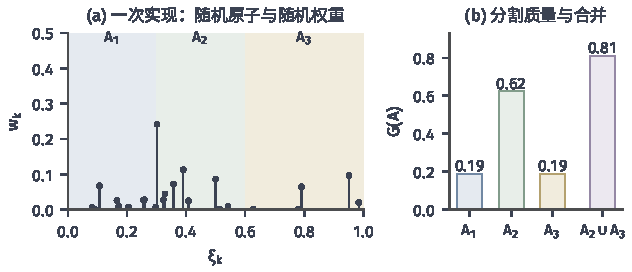
\includegraphics[width=107mm]{figures/03-optimization-evolution-and-signals/02-processes-and-trajectory-evolution/matplotlib/spp-random-measure-partition/figure.pdf}
  \caption{一个随机离散概率测度的一次实现。原子$\xi_k$独立服从$[0,1]$上的均匀分布，权重$w_k$由浓度参数$\alpha=5$的折棒构造产生（第~\ref{sec:spp-dirichlet-process}小节），共生成$400$个原子，图(a)只画出权重大于$10^{-3}$者（固定随机种子）。(b)分割$A_1=[0,0.3)$、$A_2=[0.3,0.6)$、$A_3=[0.6,1]$上的质量，以及合并$A_2\cup A_3$后的质量：合并分块时质量相加。}
  \label{fig:spp-random-measure-partition}
\end{figure}

\paragraph{评价$\sigma$代数与随机概率测度}
要把“随机的概率测度”当作一个随机对象，需要在概率测度的集合上规定$\sigma$代数。记$\mathcal P(E)$为$(E,\mathcal E)$上全体概率测度。对每个$A\in\mathcal E$，评价映射$\operatorname{ev}_A:\nu\mapsto\nu(A)$把一个概率测度映为一个数。使所有评价映射可测的最小$\sigma$代数称为\term{评价$\sigma$代数}（evaluation sigma-algebra）。

\begin{definition}[随机概率测度]
\label{def:spp-random-probability-measure}
从概率空间$(\Omega,\mathcal F,\mathbb P)$到$\mathcal P(E)$（配评价$\sigma$代数）的可测映射$G$称为$E$上的随机概率测度。
\end{definition}

这个定义可以逐个集合检查：$G$可测，当且仅当对每个$A\in\mathcal E$，$\omega\mapsto G(\omega)(A)$是随机变量。必要性是因为$\operatorname{ev}_A\circ G$是可测映射的复合；充分性的论证与定理~\ref{thm:spp-path-law}(1)相同，因为评价$\sigma$代数由集合$\operatorname{ev}_A^{-1}(B)$生成，而它们的原像$\{G(A)\in B\}$都属于$\mathcal F$。按此判据，式~\eqref{eq:spp-random-discrete}在零概率例外事件上另行指定为某个固定的概率测度后，就是一个随机概率测度。

\paragraph{三类对象的区别}
随机概率测度容易与几种相近对象混淆，它们的随机性来源与极限行为不同。

第一类是固定总体的\term{经验测度}（empirical measure）。设$X_1,X_2,\ldots$独立同分布于固定的概率测度$\nu$，$\nu_n=\frac1n\sum_{i=1}^n\delta_{X_i}$。$\nu_n$也是随机概率测度，但它的随机性只来自抽样；对每个$A$，由强大数律，$\nu_n(A)\to\nu(A)$几乎必然成立，极限是确定的。

第二类是de Finetti定理中的$\Xi$。可交换序列的经验测度$\frac1n\sum_{i\le n}\delta_{X_i}$在每个集合上也收敛，但极限$\Xi(A)$本身是随机的。随机概率测度的建模任务正是给$\Xi$指定一个分布。

第三类是以集合为索引的实值过程$(G(A))_{A\in\mathcal E}$。随机概率测度当然可以这样看，但它多了一项跨越大量坐标的约束：每次实现都要对一切可数不交并满足可数可加性。只规定每个坐标或每组有限个坐标的分布，并不自动保证这一点。

\paragraph{有限分割上的质量向量}
取$E$的有限可测分割$(A_1,\ldots,A_K)$，即两两不交、并为$E$的可测集。随机概率测度在这个分割上的质量向量$(G(A_1),\ldots,G(A_K))$取值于单纯形$\Delta_K=\{\bm p\in[0,1]^K:\ \sum_kp_k=1\}$。不同分割的质量向量之间有确定的联系：若把$A_2,A_3$合并，新分割的质量向量是$(G(A_1),G(A_2)+G(A_3),G(A_4),\ldots)$，即原向量在“相应坐标求和”这一线性映射下的像。所以，若要通过有限分割来规定随机概率测度的分布，所给的一族分割分布必须在合并下相容：细分割的分布经求和映射推送后，等于粗分割的分布。

\paragraph{相容性不足以保证可数可加}
设我们为每个有限分割规定了一个相容的质量向量分布。把可测集族$\mathcal E$当作索引集，用Kolmogorov扩张定理可以得到一族随机变量$(G(A))_{A\in\mathcal E}$，具有这些有限维分布。由相容性，对每一对固定的不交集合$A,B$，$G(A\cup B)=G(A)+G(B)$几乎必然成立；但例外的零概率事件依赖于$(A,B)$。不交集合对乃至不交集合列一般有不可数多个，零概率事件的不可数并不必是零概率事件，所以不能断言几乎每次实现都是测度。这与第~\ref{sec:spp-versions}小节“版本与不可区分”的困难同出一源。

解决的途径有两条。一条是先在一个可数的生成代数上工作，在那里可数多个零概率例外的并仍为零概率，再借助空间的正则性把有限可加的集函数延拓为测度。另一条是直接写出一个每次实现都是概率测度的构造，再验证它的有限分割规律。下一小节采用后一条途径：式~\eqref{eq:spp-random-discrete}已经保证每次实现是概率测度，只需选好权重与原子。

\subsection{Dirichlet过程的构造}
\label{sec:spp-dirichlet-process}

\paragraph{Gamma、Beta与Dirichlet质量向量}
要指定有限分割上的质量向量，需要单纯形上的一族分布，并且在合并坐标时保持同一形式。Dirichlet分布正好具备这一性质，下面用独立Gamma变量的归一化来定义它，相应的性质都可以直接推出。参数为$a>0$的\term{Gamma分布}（Gamma distribution）具有密度$y^{a-1}e^{-y}/\Gamma(a)$，$y>0$。

\begin{definition}[Dirichlet分布与Beta分布]
\label{def:spp-dirichlet-distribution}
设$\alpha_1,\ldots,\alpha_K>0$，$K\ge2$，$Y_1,\ldots,Y_K$相互独立，$Y_k$服从参数为$\alpha_k$的Gamma分布，$S=\sum_kY_k$。随机向量$(Y_1/S,\ldots,Y_K/S)$的分布称为参数为$(\alpha_1,\ldots,\alpha_K)$的\term{Dirichlet分布}（Dirichlet distribution），记作$\operatorname{Dir}(\alpha_1,\ldots,\alpha_K)$。$K=2$时第一个坐标的分布称为\term{Beta分布}（Beta distribution）$\operatorname{Beta}(\alpha_1,\alpha_2)$。约定某个参数为$0$时，相应坐标恒为$0$，其余坐标服从删去该参数后的Dirichlet分布。
\end{definition}

\begin{lemma}[Gamma归一化]
\label{lem:spp-gamma-normalization}
在上述定义中，$\bm P=(Y_1/S,\ldots,Y_K/S)$与$S$相互独立，$S$服从参数为$\alpha=\sum_k\alpha_k$的Gamma分布，$\bm P$的前$K-1$个坐标具有密度
\[
  \frac{\Gamma(\alpha)}{\prod_k\Gamma(\alpha_k)}\prod_{k=1}^Kp_k^{\alpha_k-1},\qquad p_K=1-\sum_{k<K}p_k ,
\]
定义在$\{p_k>0,\ \sum_{k<K}p_k<1\}$上。
\end{lemma}

\begin{proof}
$(Y_1,\ldots,Y_K)$的联合密度为$\prod_ky_k^{\alpha_k-1}e^{-y_k}/\Gamma(\alpha_k)$。作变量替换$s=\sum_ky_k$，$p_k=y_k/s$（$k<K$），反变换为$y_k=sp_k$（$k<K$），$y_K=s(1-\sum_{k<K}p_k)$，Jacobian行列式的绝对值为$s^{K-1}$。代入得新变量的联合密度
\[
  \frac{s^{\alpha-1}e^{-s}}{\Gamma(\alpha)}\cdot\frac{\Gamma(\alpha)}{\prod_k\Gamma(\alpha_k)}\prod_kp_k^{\alpha_k-1},
\]
它分解为$s$的函数与$\bm p$的函数之积，第一个因子是Gamma密度。所以二者独立，边缘密度如所述。
\end{proof}

由引理可以读出后面要用的三条性质。第一，合并坐标时参数相加：独立Gamma变量之和$Y_2+Y_3$仍服从Gamma分布，参数为$\alpha_2+\alpha_3$（对$(Y_2,Y_3)$用引理中$S$的分布即可），所以合并$\operatorname{Dir}(\alpha_1,\ldots,\alpha_K)$的第$2$、$3$个坐标，得到$\operatorname{Dir}(\alpha_1,\alpha_2+\alpha_3,\alpha_4,\ldots)$。第二，每个坐标的边缘分布是$\operatorname{Beta}(\alpha_k,\alpha-\alpha_k)$，把其余坐标全部合并即得。第三，$\operatorname{Beta}(a,b)$的均值为$a/(a+b)$，方差为$ab/\bigl((a+b)^2(a+b+1)\bigr)$。

\paragraph{Dirichlet过程的定义}
合并下参数相加，正是有限分割分布相容所需要的。于是可以用全体有限分割来规定一个随机概率测度的分布。

\begin{definition}[Dirichlet过程]
\label{def:spp-dirichlet-process}
设$(E,\mathcal E)$是标准Borel空间，$G_0$是其上的概率测度，$\alpha>0$。随机概率测度$G$称为参数为$(\alpha,G_0)$的\term{Dirichlet过程}（Dirichlet process），记作$G\sim\operatorname{DP}(\alpha,G_0)$，若对$E$的每个有限可测分割$(A_1,\ldots,A_K)$，
\[
  \bigl(G(A_1),\ldots,G(A_K)\bigr)\sim\operatorname{Dir}\bigl(\alpha G_0(A_1),\ldots,\alpha G_0(A_K)\bigr).
\]
$\alpha$称为\term{浓度参数}（concentration parameter），$G_0$称为\term{基测度}（base measure）。
\end{definition}

这个定义自洽：同一个粗分割可以由不同的细分割合并而得，由第一条性质，所得分布都是用粗分割的参数$\alpha G_0(\cdot)$给出的Dirichlet分布。它也唯一地确定了$G$的分布：评价$\sigma$代数上的分布由有限个评价$(G(B_1),\ldots,G(B_m))$的联合分布决定，而任意有限个集合$B_1,\ldots,B_m$生成的有限代数有一个由“原子”组成的分割，每个$G(B_i)$都是这些原子质量之和。剩下的是存在性，这正是上一小节末尾的困难。Ferguson最初提出这一定义并证明了存在性\scite{statistics-ferguson1973dirichlet}；下面给出一个每次实现都是概率测度的直接构造。

\paragraph{折棒构造}
想象一根长为$1$的木棒。先折下比例为$V_1$的一段作为第一个权重，在剩下的部分中再折下比例$V_2$作为第二个权重，如此继续：
\begin{equation}
  w_1=V_1,\qquad w_k=V_k\prod_{j<k}(1-V_j),\quad k\ge2,
  \label{eq:spp-stick-breaking}
\end{equation}
其中$V_1,V_2,\ldots$独立服从$\operatorname{Beta}(1,\alpha)$。再取与$(V_k)$独立、独立同分布于$G_0$的原子$\xi_1,\xi_2,\ldots$，按式~\eqref{eq:spp-random-discrete}定义$G$。这称为\term{折棒构造}（stick-breaking construction）。$V_k$的均值为$1/(1+\alpha)$：$\alpha$小时每次折下的比例大，质量集中在少数几个原子上；$\alpha$大时每次只折下一小段，质量分散到许多原子上。图~\ref{fig:spp-stick-breaking}(a)画出三个$\alpha$下的前$40$段，(b)画出期望权重
\[
  \mathbb Ew_k=\frac1{1+\alpha}\Bigl(\frac\alpha{1+\alpha}\Bigr)^{k-1}
\]
的几何衰减，这里用了$V_k$的独立性与$\mathbb E(1-V_j)=\alpha/(1+\alpha)$。

\begin{figure}[htbp]
  \centering
  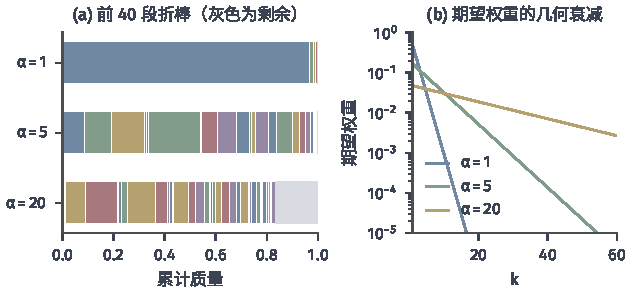
\includegraphics[width=107mm]{figures/03-optimization-evolution-and-signals/02-processes-and-trajectory-evolution/matplotlib/spp-stick-breaking/figure.pdf}
  \caption{折棒构造$w_1=V_1$，$w_k=V_k\prod_{j<k}(1-V_j)$，$V_k$独立服从$\operatorname{Beta}(1,\alpha)$。(a)$\alpha=1,5,20$各一次实现的前$40$段（颜色循环只用于区分相邻段，固定随机种子），灰色为前$40$段之后的剩余质量。(b)期望权重$\mathbb Ew_k=(1+\alpha)^{-1}\bigl(\alpha/(1+\alpha)\bigr)^{k-1}$（对数纵轴）。}
  \label{fig:spp-stick-breaking}
\end{figure}

首先要确认折下的各段加起来确实是整根木棒。记剩余长度$R_n=\prod_{j\le n}(1-V_j)$。由归纳，$\sum_{k\le n}w_k=1-R_n$：$n=1$时成立，且$1-R_n+w_{n+1}=1-R_n+V_{n+1}R_n=1-R_{n+1}$。

\begin{lemma}[剩余质量趋于零]
\label{lem:spp-stick-remainder}
$R_n\to0$几乎必然成立，从而$\sum_{k\ge1}w_k=1$几乎必然成立。
\end{lemma}

\begin{proof}
$R_n$非负且关于$n$不增，几乎必然收敛到某个$R_\infty\ge0$。由独立性，$\mathbb ER_n=\prod_{j\le n}\mathbb E(1-V_j)=\bigl(\alpha/(1+\alpha)\bigr)^n$。又$R_\infty\le R_n$，所以$\mathbb ER_\infty\le\bigl(\alpha/(1+\alpha)\bigr)^n$对每个$n$成立，$\mathbb ER_\infty=0$。非负随机变量的期望为零，它几乎必然为零。
\end{proof}

在$\sum_kw_k=1$的事件上按式~\eqref{eq:spp-random-discrete}定义$G$，在其补集这个零概率事件上令$G=G_0$。由上一小节，这样得到的$G$是随机概率测度，并且每次实现都是概率测度。

\paragraph{有限分割的Dirichlet规律}
剩下要证明折棒构造给出的$G$确实是Dirichlet过程。证明的想法来自一个自相似性：折下第一段后，剩下的部分按同样的规则继续折，所以$G$等于“一个原子的质量$V_1$”加上“比例为$1-V_1$的一个同分布的随机测度”。若Dirichlet分布在这一操作下保持不变，再加上剩余质量趋于零，就能推出结论。这一构造由Sethuraman提出。

\begin{theorem}[折棒构造给出Dirichlet过程]
\label{thm:spp-stick-breaking-dp}
设$V_k$独立服从$\operatorname{Beta}(1,\alpha)$，$\xi_k$独立同分布于$G_0$且与$(V_k)$独立，$G$由式~\eqref{eq:spp-stick-breaking}与式~\eqref{eq:spp-random-discrete}定义（在零概率例外事件上令$G=G_0$）。则$G\sim\operatorname{DP}(\alpha,G_0)$。
\end{theorem}

\begin{proof}
固定有限可测分割$(A_1,\ldots,A_K)$，记$g_i=G_0(A_i)$。若某个$g_i=0$，则几乎必然没有原子落入$A_i$，$G(A_i)=0$，符合零参数的约定；删去这些分块后，不妨设所有$g_i>0$，$K\ge2$（$K=1$时结论平凡）。令$J_k$为$\xi_k$所在分块的编号，则$J_1,J_2,\ldots$独立同分布，$\mathbb P(J_k=i)=g_i$，且与$(V_k)$独立。记$\bm e_i$为第$i$个标准单位向量，质量向量可以写成
\[
  \bm P=\bigl(G(A_1),\ldots,G(A_K)\bigr)=\sum_{k\ge1}w_k\bm e_{J_k}.
\]
记$\bm g=(g_1,\ldots,g_K)$，目标是证明$\bm P\sim\operatorname{Dir}(\alpha\bm g)$。

第一步，一步不变性：若$\bm Q\sim\operatorname{Dir}(\alpha\bm g)$，$V\sim\operatorname{Beta}(1,\alpha)$，$J$以概率$g_i$取$i$，三者独立，则$V\bm e_J+(1-V)\bm Q\sim\operatorname{Dir}(\alpha\bm g)$。先固定$J=i$。取相互独立的$Y_0$（Gamma参数$1$）与$Y_1,\ldots,Y_K$（Gamma参数$\alpha g_1,\ldots,\alpha g_K$），令$\Sigma=\sum_{l\ge1}Y_l$。由引理~\ref{lem:spp-gamma-normalization}，$(Y_l/\Sigma)_l\sim\operatorname{Dir}(\alpha\bm g)$且与$\Sigma$独立，也与$Y_0$独立；$\Sigma$的参数为$\alpha$，所以$Y_0/(Y_0+\Sigma)\sim\operatorname{Beta}(1,\alpha)$，并且它与$(Y_l/\Sigma)_l$独立。于是$(V,\bm Q)$与$\bigl(Y_0/(Y_0+\Sigma),(Y_l/\Sigma)_l\bigr)$同分布，
\[
  V\bm e_i+(1-V)\bm Q\overset{\mathrm d}{=}\frac{Y_0\bm e_i+(Y_1,\ldots,Y_K)}{Y_0+\Sigma}\sim\operatorname{Dir}(\alpha\bm g+\bm e_i),
\]
因为第$i$个分子$Y_0+Y_i$服从参数为$\alpha g_i+1$的Gamma分布，且各分子仍独立。再对$J$平均。由引理中的密度，并利用$\Gamma(\alpha+1)=\alpha\Gamma(\alpha)$与$\Gamma(\alpha g_i+1)=\alpha g_i\Gamma(\alpha g_i)$，$\operatorname{Dir}(\alpha\bm g+\bm e_i)$的密度等于$\operatorname{Dir}(\alpha\bm g)$的密度$D(\bm p)$乘以$\frac{\alpha}{\alpha g_i}p_i=p_i/g_i$。所以混合的密度为
\[
  \sum_{i=1}^Kg_i\cdot\frac{p_i}{g_i}D(\bm p)=\Bigl(\sum_ip_i\Bigr)D(\bm p)=D(\bm p),
\]
即$V\bm e_J+(1-V)\bm Q\sim\operatorname{Dir}(\alpha\bm g)$。

第二步，有限步迭代。取$\bm Q_0\sim\operatorname{Dir}(\alpha\bm g)$，与全部$(V_k,J_k)$独立，令
\[
  \bm P^{(n)}=\sum_{k\le n}w_k\bm e_{J_k}+R_n\bm Q_0 .
\]
它可以写成$\bm P^{(n)}=V_1\bm e_{J_1}+(1-V_1)\bm P'^{(n-1)}$，其中$\bm P'^{(n-1)}$是用$(V_2,\ldots,V_n)$、$(J_2,\ldots,J_n)$与$\bm Q_0$按同样公式构成的向量，与$(V_1,J_1)$独立。对$n$归纳：$\bm P^{(0)}=\bm Q_0\sim\operatorname{Dir}(\alpha\bm g)$；若$n-1$步的向量服从$\operatorname{Dir}(\alpha\bm g)$，则$\bm P'^{(n-1)}$也服从它，由第一步，$\bm P^{(n)}\sim\operatorname{Dir}(\alpha\bm g)$。

第三步，取极限。在$\sum_kw_k=1$的事件上，$\bm P-\bm P^{(n)}=\sum_{k>n}w_k\bm e_{J_k}-R_n\bm Q_0$，每个坐标的绝对值不超过$\sum_{k>n}w_k+R_n=2R_n$。由引理~\ref{lem:spp-stick-remainder}，$\bm P^{(n)}\to\bm P$几乎必然成立，从而依分布收敛；而每个$\bm P^{(n)}$的分布都是$\operatorname{Dir}(\alpha\bm g)$，所以$\bm P\sim\operatorname{Dir}(\alpha\bm g)$。
\end{proof}

\paragraph{浓度参数与基测度的作用}
由Beta边缘的均值与方差公式，对每个可测集$A$，
\[
  \mathbb EG(A)=G_0(A),\qquad \operatorname{Var}G(A)=\frac{G_0(A)\bigl(1-G_0(A)\bigr)}{1+\alpha}.
\]
基测度$G_0$决定随机测度的平均形状，浓度参数$\alpha$决定它围绕平均形状的离散程度。图~\ref{fig:spp-dp-samples}以$G_0=\mathcal N(0,1)$画出随机分布函数$G((-\infty,x])$的样本：$\alpha=1$时，几个大原子造成少数几级大台阶，样本与$G_0$相去甚远；$\alpha=100$时，样本紧贴$G_0$的分布函数。

\begin{figure*}[htbp]
  \centering
  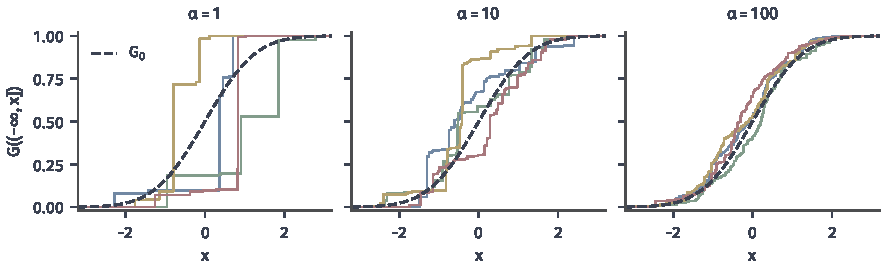
\includegraphics[width=150mm]{figures/03-optimization-evolution-and-signals/02-processes-and-trajectory-evolution/matplotlib/spp-dp-samples/figure.pdf}
  \caption{Dirichlet过程$\operatorname{DP}(\alpha,\mathcal N(0,1))$的随机分布函数$x\mapsto G((-\infty,x])$。每幅图画四次独立实现（彩色阶梯线，由折棒构造截断到$6000$个原子生成，截断后剩余质量可忽略，固定随机种子），虚线为基测度$\mathcal N(0,1)$的分布函数。浓度参数从左到右为$\alpha=1,10,100$。}
  \label{fig:spp-dp-samples}
\end{figure*}

无论$G_0$是否连续，折棒构造的每次实现都是离散测度。这在抽样时有一个直接后果。给定$G$，独立抽取$X_1,X_2\sim G$；若$G_0$没有原子，则不同的$\xi_k$几乎必然互不相同，$X_1=X_2$当且仅当两次抽到同一个原子，于是
\[
  \mathbb P(X_1=X_2)=\mathbb E\sum_kw_k^2=\frac1{1+\alpha}.
\]
最后一个等式的计算如下：$\mathbb EV^2=2/\bigl((1+\alpha)(2+\alpha)\bigr)$，$\mathbb E(1-V)^2=\alpha/(2+\alpha)$，由独立性
\[
  \mathbb E\sum_kw_k^2=\mathbb EV^2\sum_{k\ge1}\bigl(\mathbb E(1-V)^2\bigr)^{k-1}=\frac{2}{(1+\alpha)(2+\alpha)}\cdot\frac{2+\alpha}2=\frac1{1+\alpha}.
\]
$\alpha$越小，重复抽到同一个值的概率越大。由de Finetti定理的反向结论，给定$G$后条件独立抽取的$X_1,X_2,\ldots$构成一个可交换序列，它的随机背景$\Xi$就是$G$；这把本节与上一节连在一起。这种重复取值的结构是Dirichlet过程用于聚类的出发点。

有限Dirichlet分布族的系统性质由卷四的概率分布部分处理；给定观测后Dirichlet过程的后验、由重复取值导出的聚类表示以及非参数推断，则由卷四的统计推断部分处理。

% 第4章小结。

\section{本章小结}
\label{sec:spp-summary}

章首的四类问题对应同一个过程的四个描述层次。固定一个时刻，过程是一个随机变量，回答单个时刻的读数可能是什么。固定有限个时刻，有限维分布记录它们的共同变化；相同边缘、不同相关的三个序列表明，平均值能否收敛、收敛多快都取决于这一层，而不取决于单时刻分布。固定一次实现，样本路径回答整条曲线的形状；在乘积$\sigma$代数中，全部有限维分布与路径规律是同一份信息，但其中每个事件只依赖可数个坐标，所以连续时间下“路径是否连续”“全程上确界多大”这类问题不能只靠有限维分布提出。最后，滤过规定每个时刻已经可以判定的事件：适应性要求当前值已知，停时要求停止决定不偷看未来。同一个过程相对于不同的滤过可以有不同的预测和不同的性质，所以鞅与Markov性质都必须连同滤过一起陈述；停时的定义也不保证停止后的期望等式，倍投策略说明需要另加条件。

构造过程有两条路线，分别对应有无时间顺序。有时间顺序时，初始分布加上依赖历史的概率核逐步给出有限路径的分布，核的归一化自动保证相容，Ionescu-Tulcea定理把它们拼成无穷序列的规律，且不需要拓扑条件；在标准Borel空间上，序列规律与“初始分布加条件核”是等价的描述。没有时间顺序时，给出全体有限子集上的相容分布族，Kolmogorov扩张定理在标准Borel状态空间上给出乘积空间上唯一的规律；两两相容而不存在三元规律的例子提醒我们，每个有限子集上都必须给出真正的概率测度。扩张定理交付的是坐标族，不是路径性质。版本与不可区分把“同一个过程”的两种含义分开：随机位置的尖点说明，不可数索引下二者确实不同，有限维分布不能决定路径是否连续；右连续性让可数个时刻代替全部时刻，连续版本因此在不可区分意义下唯一。Kolmogorov连续性准则用增量矩的幂次条件给出连续版本和Hölder指数，增量矩随间隔的标度把Brownian运动与Poisson计数过程区分开来。

后三节把索引推广到一般位置和集合。高斯过程的全部规律由均值函数与半正定协方差函数决定，半正定性既是必要条件也是充分条件；路径的正则性由增量方差的衰减控制，而同一个核作为再生核所定义的Hilbert空间描述的是确定性函数，Brownian路径几乎必然不在其中。交换序列的依赖来自共享的随机背景：交换性与独立、与平稳各约束联合规律的不同方面，de Finetti定理表明无限可交换序列就是“先抽随机分布、再条件独立抽样”，经验频率收敛到一个随机的极限。随机概率测度的每次实现本身是一个概率分布；有限分割上的相容规律不足以保证每次实现都可数可加，折棒构造给出了每次实现都是概率测度的Dirichlet过程，浓度参数与基测度分别控制离散程度与平均形状。

后两章按时间索引组织。第~\ref{chap:discrete-time-stochastic-processes}章在离散时间中使用本章的逐步核构造、滤过与停时，研究转移、累计、停止与长期行为；离散索引下版本与不可区分没有区别，乘积$\sigma$代数已经包含所需的路径事件。第~\ref{chap:continuous-time-stochastic-processes}章面对不可数时刻，需要本章的连续版本、联合可测性与路径正则性，并在相应问题处补充滤过的右连续性、可积性与过程列的统一控制等新条件。Markov性质、鞅性质与平稳性是可以同时成立的性质，不是互斥的过程类别。本章的高斯过程、交换序列与随机概率测度展示了构造的思路，但不是后两章每个结果的前提。

